%% Based on a TeXnicCenter-Template by Gyorgy SZEIDL.
%%%%%%%%%%%%%%%%%%%%%%%%%%%%%%%%%%%%%%%%%%%%%%%%%%%%%%%%%%%%%

%----------------------------------------------------------
%
\documentclass{book}%
%
%----------------------------------------------------------
% This is a sample document for the standard LaTeX Book Class
% Class options
%       --  Body text point size:
%                        10pt (default), 11pt, 12pt
%       --  Paper size:  letterpaper (8.5x11 inch, default)
%                        a4paper, a5paper, b5paper,
%                        legalpaper, executivepaper
%       --  Orientation (portrait is the default):
%                        landscape
%       --  Printside:   oneside, twoside (default)
%       --  Quality:     final(default), draft
%       --  Title page:  titlepage, notitlepage
%       --  Columns:     onecolumn (default), twocolumn
%       --  Start chapter on left:
%                        openright(no, default), openany
%       --  Equation numbering (equation numbers on right is the default):
%                        leqno
%       --  Displayed equations (centered is the default):
%                        fleqn (flush left)
%       --  Open bibliography style (closed bibliography is the default):
%                        openbib
% For instance the command
%          \documentclass[a4paper,12pt,reqno]{book}
% ensures that the paper size is a4, fonts are typeset at the size 12p
% and the equation numbers are on the right side.
%

%%%%%%%%%%%%%%%%%%%%%%
%% PACKAGES
%%%%%%%%%%%%%%%%%%%%%%
\usepackage{amsmath}
%\usepackage[super,square,comma]{natbib}
\usepackage[twoside,letterpaper,width=6in,height=8in]{geometry}
\usepackage{siunitx} % format units properly
\usepackage{wrapfig}
\usepackage[margin=10pt,font=small,labelfont=bf]{caption} % format captions
\usepackage{booktabs} % nicer tables
\usepackage{subcaption} 
\usepackage{csquotes} % block quotes
\usepackage{tikz}
\usepackage[inline, shortlabels]{enumitem} % inline enumeration

\usepackage{graphicx} % packages are used to modify the text and create bling.
\usepackage{gensymb}
\usepackage{natbib}
\usepackage{glossaries}

%\usepackage[usenames]{xcolor}% for commenting in color!
\bibliographystyle{ecology}

\RequirePackage{hyperref} % For hyperlinked cross-references
\hypersetup{
    colorlinks,
    citecolor=blue,
    filecolor=blue,
    linkcolor=blue,
    urlcolor=blue
}

\usepackage{amsmath}%
\usepackage{amsfonts}%
\usepackage{amssymb}%
\usepackage{graphicx}
%----------------------------------------------------------
\newtheorem{theorem}{Theorem}
\newtheorem{acknowledgement}[theorem]{Acknowledgement}
\newtheorem{algorithm}[theorem]{Algorithm}
\newtheorem{axiom}[theorem]{Axiom}
\newtheorem{case}[theorem]{Case}
\newtheorem{claim}[theorem]{Claim}
\newtheorem{conclusion}[theorem]{Conclusion}
\newtheorem{condition}[theorem]{Condition}
\newtheorem{conjecture}[theorem]{Conjecture}
\newtheorem{corollary}[theorem]{Corollary}
\newtheorem{criterion}[theorem]{Criterion}
\newtheorem{definition}[theorem]{Definition}
\newtheorem{example}[theorem]{Example}
\newtheorem{exercise}[theorem]{Exercise}
\newtheorem{lemma}[theorem]{Lemma}
\newtheorem{notation}[theorem]{Notation}
\newtheorem{problem}[theorem]{Problem}
\newtheorem{proposition}[theorem]{Proposition}
\newtheorem{remark}[theorem]{Remark}
\newtheorem{solution}[theorem]{Solution}
\newtheorem{summary}[theorem]{Summary}
\newenvironment{proof}[1][Proof]{\textbf{#1.} }{\ \rule{0.5em}{0.5em}}
%----------------------------------------------------------

\graphicspath{{graphics/}}

\title{Environmental Science: East Asia and the World}
\author{EnviroLab Asia Fellows}

\makeatletter
\newcommand{\chapterauthor}[1]{%
  {\parindent0pt\vspace*{-25pt}%
  \linespread{1.1}\large\scshape#1%
  \par\nobreak\vspace*{35pt}}
  \@afterheading%
}
\makeatother



\title{Environmental Science: East Asia and the World}
\author{EnviroLab Asia Fellows}

\makeglossaries

\begin{document}

\frontmatter

\maketitle
\tableofcontents

\chapter*{Preface}

\section{Guiding Principles}

In this project, the EnviroLab Asia fellows have written a textbook that highlights examples of environmental processes that occur along a vertical axis. 

Each student contributes to one theme, composed of two examples that highlight environmental issues of East Asia. However, our goal is not to blame East Asian, but to point to linkages of how a range of globalized economy contribute to these environmental problems. 

In the end, it would be useful for us to acknowledge we have some capacity to address these how these global linkages could be modified to reduce these environmental issues. 

\subsection{Goals}

Processes across horizontal boundaries define many environmental patterns that frame human interactions with the environment. How do humans impact processes that cross these boundaries and how do humans influence these ecosystem interface?

\subsection{Rationale}

\subsection{Activity}

Each group will be composed of two students, that will become experts and teach their classmates on the topic. 

\section{East Asia and the World}







\section{Acknowledgments}

Everyone in the world!



\section{Setting Up Book Project--Type Setting w/ \LaTeX}

\subsection{The Standard Latex Book Class}


\section{The Most Important Features of this Document}

\section{Section}

Use the \verb"\section{Section}" command for major sections, and the
\verb"\subsection{Subsection}" command for subsections, etc.

\subsection{Subsection}

This is just some text under a subsection.

\subsubsection{Subsubsection}

This is just some text under a subsubsection.

\paragraph{Subsubsubsection}

This is just some  text under a subsubsubsection.

\subparagraph{Subsubsubsubsection}

This is just some text under a subsubsubsubsection.

\section{Typesetting Commands}

SSelect a part of the text then click on the button Emphasize (H!), or Bold (Fs), or
Italic (Kt), or Slanted (Kt) to typeset \emph{Emphasize}, \textbf{Bold},
\textit{Italics}, \textsl{Slanted} texts.

You can also typeset \textrm{Roman}, \textsf{Sans Serif}, \textsc{Small Caps}, and
\texttt{Typewriter} texts.

You can also apply the special, mathematics only commands $\mathbb{BLACKBOARD}$
$\mathbb{BOLD}$, $\mathcal{CALLIGRAPHIC}$, and $\mathfrak{fraktur}$. Note that
blackboard bold and calligraphic are correct only when applied to uppercase letters A
through Z.

You can apply the size tags -- Format menu, Font size submenu -- {\tiny tiny},
{\scriptsize scriptsize}, {\footnotesize footnotesize}, {\small small}, {\normalsize
normalsize}, {\large large}, {\Large Large}, {\LARGE LARGE}, {\huge huge} and {\Huge
Huge}.

You can use the \verb"\begin{quote} etc. \end{quote}" environment for typesetting
short quotations. Select the text then click on Insert, Quotations, Short Quotations:

\begin{quote}
The buck stops here. \emph{Harry Truman}

Ask not what your country can do for you; ask what you can do for your
country. \emph{John F Kennedy}

I am not a crook. \emph{Richard Nixon}

I did not have sexual relations with that woman, Miss Lewinsky. \emph{Bill Clinton}
\end{quote}

The Quotation environment is used for quotations of more than one paragraph. Following
is the beginning of \emph{The Jungle Books} by Rudyard Kipling. (You should select
the text first then click on Insert, Quotations, Quotation):

\begin{quotation}
It was seven o'clock of a very warm evening in the Seeonee Hills when Father Wolf woke
up from his day's rest, scratched himself, yawned  and spread out his paws one after
the other to get rid of sleepy feeling in their tips. Mother Wolf lay with her big gray
nose dropped across her four tumbling, squealing cubs, and the moon shone into the
mouth of the cave where they all lived. ``\emph{Augrh}'' said Father Wolf, ``it is time
to hunt again.'' And he was going to spring down hill when a little shadow with a bushy
tail crossed the threshold and whined: ``Good luck go with you, O Chief of the Wolves;
and good luck and strong white teeth go with the noble children, that they may never
forget the hungry in this world.''

It was the jackal---Tabaqui the Dish-licker---and the wolves of India despise Tabaqui
because he runs about making mischief, and telling tales, and eating rags and pieces of
leather from the village rubbish-heaps. But they are afraid of him too, because
Tabaqui, more than any one else in the jungle, is apt to go mad, and then he forgets
that he was afraid of anyone, and runs through the forest biting everything in his way.
\end{quotation}

Use the Verbatim environment if you want \LaTeX\ to preserve spacing, perhaps when
including a fragment from a program such as:
\begin{verbatim}
#include <iostream>         // < > is used for standard libraries.
void main(void)             // ''main'' method always called first.
{
 cout << ''This is a message.'';
                            // Send to output stream.
}
\end{verbatim}
(After selecting the text click on Insert, Code Environments, Code.)


\section{Mathematics and Text}

It holds \cite{KarelRektorys} the following
\begin{theorem}
(The Currant minimax principle.) Let $T$ be completely continuous selfadjoint operator
in a Hilbert space $H$. Let $n$ be an arbitrary integer and let $u_1,\ldots,u_{n-1}$ be
an arbitrary system of $n-1$ linearly independent elements of $H$. Denote
\begin{equation}
\max_{\substack{v\in H, v\neq
0\\(v,u_1)=0,\ldots,(v,u_n)=0}}\frac{(Tv,v)}{(v,v)}=m(u_1,\ldots, u_{n-1})
\label{eqn10}
\end{equation}
Then the $n$-th eigenvalue of $T$ is equal to the minimum of these maxima, when
minimizing over all linearly independent systems $u_1,\ldots u_{n-1}$ in $H$,
\begin{equation}
\mu_n = \min_{\substack{u_1,\ldots, u_{n-1}\in H}} m(u_1,\ldots, u_{n-1}) \label{eqn20}
\end{equation}
\end{theorem}
The above equations are automatically numbered as equation (\ref{eqn10}) and
(\ref{eqn20}).


\section{Lists Environments}

You can create numbered, bulleted, and description lists
(Use the Itemization or Enumeration buttons, or click on the Insert menu
then chose an item from the Enumeration submenu):

\begin{enumerate}
\item List item 1

\item List item 2

\begin{enumerate}
\item A list item under a list item.

\item Just another list item under a list item.

\begin{enumerate}
\item Third level list item under a list item.

\begin{enumerate}
\item Fourth and final level of list items allowed.
\end{enumerate}
\end{enumerate}
\end{enumerate}
\end{enumerate}

\begin{itemize}
\item Bullet item 1

\item Bullet item 2

\begin{itemize}
\item Second level bullet item.

\begin{itemize}
\item Third level bullet item.

\begin{itemize}
\item Fourth (and final) level bullet item.
\end{itemize}
\end{itemize}
\end{itemize}
\end{itemize}

\begin{description}
\item[Description List] Each description list item has a term followed by the
description of that term.

\item[Bunyip] Mythical beast of Australian Aboriginal legends.
\end{description}

\section{Theorem-Like Environments}

The following theorem-like environments (in alphabetical order) are available
in this style.

%\begin{acknowledgement}
%This is an acknowledgement
%\end{acknowledgement}

%\begin{algorithm}
%This is an algorithm
%\end{algorithm}

%\begin{axiom}
%This is an axiom
%\end{axiom}

%\begin{case}
%This is a case
%\end{case}

%\begin{claim}
%This is a claim
%\end{claim}

%\begin{conclusion}
%This is a conclusion
%\end{conclusion}

%\begin{condition}
%This is a condition
%\end{condition}

%\begin{conjecture}
%This is a conjecture
%\end{conjecture}

%\begin{corollary}
%This is a corollary
%\end{corollary}

%\begin{criterion}
%This is a criterion
%\end{criterion}

\newglossaryentry{peat}{
	name=peat, 
	description={peat is cool.}
}

\begin{definition}
This is a definition and the word is use in an glossary, e.g. \gls{peat}
\end{definition}



\begin{example}
This is an example
\end{example}

\begin{exercise}
This is an exercise
\end{exercise}

\begin{lemma}
This is a lemma
\end{lemma}

\begin{proof}
This is the proof of the lemma.
\end{proof}

\begin{notation}
This is notation
\end{notation}

\begin{problem}
This is a problem
\end{problem}

\begin{proposition}
This is a proposition
\end{proposition}

\begin{remark}
This is a remark
\end{remark}

\begin{summary}
This is a summary
\end{summary}

\begin{theorem}
This is a theorem
\end{theorem}

\begin{proof}
[Proof of the Main Theorem]This is the proof.
\end{proof}

\subsubsection{``Child'' Rnw Contributions}

This is a chapter that we can input into the text... you will each create a chapter without the preamble and begin and end document... that can be integrated into a single book! 

\section{Thoughts for the Contributors}

This template will NOT teach you how to use \LaTeX! To accomplish that, we'll rely on some great online resource that you can find on the project page. 

Instead this section of the document is designed to demonstrate how our textbook will look, feel, and ultimately how we contribute to the project.

This document also compiles all of our projects into a single PDF, when each ``child'' Rnw is ready to be included.

\subsection{Using Sections To Create Text Structure}

You should divide up your chapter into sections and subsections...


We may dispense with subsubsections, but for now they might be useful. We will use section, subsection, and subsubsection to break up the topic into bite sizes. 

\section{Some Type Setting Stuff}

\subsection{Making bulletted lists, enumerations...}

\begin{itemize}
\item one
\item two 
\item three
\end{itemize}

We use special commands to create an itemized list.

\subsection{Peer Review Commenting}

You can put your comments in square brackets and in color for things that need help. \textcolor{red}{[This section is confusing, I am not sure what commmenting means.]}

\subsection{Be sure to use ascII characters}

\LaTeX doesn't like a range of characters or they reserved for special behavior...

For example, the \# is used for tabs in a table environment. \% is used to make comments, thus stuff behind a \% is ignored. There are lots of others, but these come up the most.

\subsection{Creating equations}

One of the most powerful parts of \LaTeX is how it can be used to write complex equations, with all those symbols and Greek letters! This can be done inline $y = mx + b + \epsilon$ for fairly simple equations, or set apart for more complex equations:

\begin{equation}
\int_0^\infty e^{-x^2} dx=\frac{\sqrt{\pi}}{2}
\end{equation}

\section{Adding Figures, etc}

\subsection{Using Rnw Files -- Deprecated}

Originally, I used R and Rnw files that were converted to tex files, in Rstudio. However, this step was too complicated for students, so I now recommend the use of tex files and use Rstudio to create figure files as a separate process. Thus, I will no longer explain the process in this document. 

\subsection{Creating a floating figure}

This is my floating figure (Figure \ref{fig:plot}).

\begin{figure}
\label{fig:plot}
\caption{My plot's caption is here!}
\end{figure}

\section{Creating References}

\section{Bibliography generation}

This document was produced in RStudio using the knitr package \citep{knitr2013} by \url{http://texblog.org}. 

Also try \citet{fenner2018} to create an author title. 

Currently, we are using the ecology.bst, but it has trouble with misc type of references, so I will changing this in 2019. 
 
\chapter{Introduction}

The introduction is entered using the usual chapter command. Since
the introduction chapter appears before the \verb|mainmatter| TeX
field, it is again an unnumbered chapter. The primary difference
between the preface and the introduction in this sample document
is that the introduction will appear in the table of contents and
the page headings for the introduction are automatically handled
without the need for the \verb|markboth| TeX field. You may use
either or both methods to create chapters at the beginning of your
document. You may also delete these preliminary chapters.

\subsection{Guiding Principles}

In this project, the EnviroLab Asia fellows have written a textbook that highlights examples of environmental processes that occur along a vertical axis. 

Each student contributes to one theme, composed of two examples that highlight environmental issues of East Asia. However, our goal is not to blame East Asian, but to point to linkages of how a range of globalized economy contribute to these environmental problems. 

In the end, it would be useful for us to acknowledge we have some capacity to address these how these global linkages could be modified to reduce these environmental issues. 

\section{Goals}

Processes across horizontal boundaries define many environmental patterns that frame human interactions with the environment. How do humans impact processes that cross these boundaries and how do humans influence these ecosystem interface?

Non-declintionist views...but also no technological optimism. 

\subsection{Rationale}


\section{Acknowledgments}

Everyone in the world!

\subsection{Activity}

Each group will be composed of two students, that will become experts and teach their classmates on the topic. 


\section{Patterns and Processes in Scale}

\subsection{Project Themes}

How do environmental interfaces in East Asia influence human infrastructure and vice versa?

\begin{description}
	\item[A. Space-Atmosphere Interface] These might include the Earth's energy budget, drivers of climate and climate change, UV radiation and ozone processes.
	
	\item[B. Mantle-Lithosphere] The Earth's core and mantel are active agents in the definition and processes that influence tectonic and landforms -- but also frame how, where, and when natural disasters occur, but they also tell use much about the resources, fuels and ores, used in the development of modern industrialization.  
	
	\item[X. Hydrologic Cycle]	
	
	\item[D. Soil-Water-Atmosphere Interface: Plant Biomass and Diversity] Light and gas exchange are the most common discussed fluxes across the air-water interface, but various dead and living biotic material also comes from or is deposited into the water column. While rainfall drives the productivity of terrestiral plant growth, the diversity is thought to depend on a range of processes.

	\item[C. Soil-Air Interface] Pedogenesis of soils includes climate (rain, air temperatures), atmospheric deposition of dust and other particles and gas exchange. 
	
	\item[X Carbon in Air, Plants, and Soil: Peatlands]
	
	\item[E. Benthos-Water Interface] The flow of ions, organic matter deposited, gas and nutrient exchanges.

	\item[X. Isostasy and Continental Plates]
	
	\item[X. Tectonic Hazards]
	
	\item[X. Weather Patterns and the Dynamic Climate System]
	
	\item[X. Hydrologic Hazards: Floods and Droughts]
	
\end{description}	

\section{East Asia and the World}

\mainmatter
\part{Vertical Processes}

%%%%%%%%%%%%%%%%%%%%%%%%%%%%%%%
%%  CHAPTERS BY FELLOWS AND FACULTY 
%%%%%%%%%%%%%%%%%%%%%%%%%%%%%%%

\input{chapters/02_EarthSun}
\chapter{Mining in East Asia}
\chapterauthor{Alison Hong\footnote{Statement of Contributions: }}

\section{History of Mining}

\subsection{Gold in the Phillipines}

The Phillipines had the second largest gold reserve in world and employs approximately 200,000-300,000 people, most of who work in small scale mining operations, making approximately \$5/day (Pri)[??]

Many family miners, independent miners who make up the 70-80\% from small mining operations in the country. 


Large scale: \$70 billion 2014 (HWR)

90\% smuggled illegally

2015: Gov simplified process of gaining license 

\subsection{Geology and Gold}

\section{Mining and Proccesing Gold}

\subsection{Mining Methods and Ecological Impacts}

\subsection{Large Scale Processing}

\subsection{Smale Scale Operations}

\citet{drasch2001mt} \ldots

Working small scale in families... (Figure \ref{fig:famliymining}).

\begin{figure}[h]
\includegraphics[width=\textwidth]{Family_Mining_Phillipines_SourceUnknwn}
\label{fig:famliymining}
\caption{Insert Caption Here: \ldots (With Permission ??).}
\end{figure}

\citep{de2016copper}

De la Torre, JB, Claveria RJ, Perez RE, Perez TR, Doronilla Al. 2016. Copper uptake by Pteris melanocaulon Fee from a Copper-Gold mine in Surigao del Norte Philippines. CRC Press LLC. 

Saludes, Mark. September 29, 2015. Hazardous Child Labor in Small-Scale Gold Mining in the Philippines. Human Rights Watch; [September 29, 2015; February 6, 2018].

\citet{santos1974mineral}

Santos G. 1974. Mineral Distribution and Geological Features of the Philippines. In: Petrascheck W.E. (eds) Metallogenetische und Geochemische Provinzen / Metallogenetic and Geochemical Provinces. �sterreichische Akademie der Wissenschaften Schriftenreihe der Erdwissenschaftlichen Kommission, vol 1. Springer, Vienna

Wernick, Adam. June 3, 2014. In the Philippines, underwater gold mining comes with small payoffs and big risk. PRI; [June 3, 2014; February 6, 2018]. 

\citet{drasch2001mt}

\section{Asia's Appetite for Sand}

Larson, Christina. "Asia's hunger for sand takes toll on ecology." (2018): 964-965.


%\bibliography{../references}




\chapter{The Formation and Extraction of Fossil Fuels}
\chapterauthor{Eliana Goehring}                       

%%%%%%%%%%%%%%%%%%%%%%%%%%%%%
%The burning motivation
%%%%%%%%%%%%%%%%%%%%%%%%%%%%%

\section{Underground Coal Fires in China} 

Fires are burning in hundreds of underground coal deposits throughout China, releasing huge amounts of greenhouse gases, fundamentally changing landscapes, and having serious economic impacts. An estimated 15--20 million tons of coal are burning annually in northern China through these inadvertent fires. \cite{kuenzer2007uncontrolled}

Underground coal fires are not a new phenomena. Lightning strikes, grass and forest fires, and spontaneous combustion have all been contributing to coal fires for the past few million years. \cite{ceycoal} It is the frequency of these fires that has significantly increased due to human activity over the past century as more coal deposits are exposed for mining. 

As coal deposits are consumed by fires below ground, \textbf{subsidence} often becomes apparent above ground. Land subsidence refers to the gradual settling or sudden sinking of the Earth's surface. 
%%Cite USGS Groundwater Information: Land Subsidence
The landscape changes in areas surrounding subsurface coal fires are not subtle. Cracks induced by subsidence can measure up to a few meters wide, hundreds of meters deep, and can continue onward for several kilometers in length. \cite{stracher2004coal}

These cracks, which often occur on a slightly smaller scale, are part of a positive feedback loop. 
%%%Cite Colin's section about feedback%%%
As coal deposits burn below ground, they create cracks in the ground above them. This gives the fire greater access to oxygen thereby promoting combustion. Consequently the coal continues to burn, causes more subsidence, more burning, and so on. Figure~\ref{fig:undergroundfire} shows how the underground coal fires cause the ground above them to subside and greater air flow increases the fire's capabilities. 


\begin{figure}[ht]
\centering
    \includegraphics[width = 0.70\textwidth]{undergroundfire.png}
    \caption{Underground coal fire. Schematic showing subsidence and pollution that occurs with underground coal fires. }
    \label{fig:undergroundfire}
\end{figure}


Typically when fossil fuels are studied within the realm of environmental science, we focus on how relying on them for energy contributes to green house gases. In this chapter, we are going to delve into other ways in which fossil fuels affect the environment. By focusing on the extraction processes of different types of fuels, we will discover the ways in which surrounding ecosystems are directly affected by mining through land subsidence and ground water pollution. We will focus on China, as this is the largest fossil fuel producer and user in all of Asia. 


% \section{Underground Coal Fires in China} \cite{stracher2004coal}
%   \1 Cracks induced by subsidence measuring up to ``several kilometers long, tens of meters wide, and hundred of meters deep"
%       \2 Positive feedback loop- cracks increase oxygen circulation thereby promoting combustion 
%   \1 Economic loss estimated to be as high as \$25-250 million USD (Prakarsh)

% Citeint ``China: World�s Largest Energy Consumer and Greenhouse Gas Emitter"
%   \1 China 2012, coal is 66\% of energy, fossil fuels over 90\%
%   \1 China is estimated to contain over 90 billion tonnes of coal reserves. In 2016, the country produced 2.62 billion tonnes of coal. CITE(world energy council)






%%%%%%%%%%%%%%%%%%%%%%%%%%%%%
%What are fossil fuels
%%%%%%%%%%%%%%%%%%%%%%%%%%%%%

\section{Fossil Fuel Formation}

Before we can examine the ways in which fossil fuels are extracted, it is important that we understand what fossil fuels are, how they were formed, and when this all started.

\textbf{Fossil fuels} are hydrocarbons, meaning they are composed of hydrogen and carbon. This term typically includes coal, crude oil, and natural gas which all started to form millions of years ago from plant and animal remains. A combination of extremely high temperatures, high pressures, and millions of years allowed these organisms to be transformed into fossil fuels. 

\subsection{Coal Formation}

\subsubsection{Timeline}

The most significant coal formations stem from trees, ferns, and other plants that were growing during the Carboniferous ``coal-bearing" Period 290--360 million years ago. A combination of environmental factors, such as the evolution of large woody trees, allowed for coal deposits to begin to form during this time period. Lesser formations of coal continued through the Permian and Mesozoic Eras, 290--250 and 250--65 million years ago, respectively. Coal deposits that are less than 65 million years in age typically yield low quality coal, as they have not have enough time to fully transform into high-grade coal. 



\subsubsection{Process}


The first trees evolved around 360 million years ago at the beginning of the Carboniferous period. These ancient trees are the basis for our coal.  Coal formation begins with thousands of years of plant accumulation. This process starts with plants in wetland environments dying and beginning to decompose. This plant matter is then buried beneath new layers of plants which later die and add to the layers of organic matter beneath them. The resulting partially decomposed plant matter is known as \textbf{peat}. In tropical climates, the rate of peat accumulation is estimated to be about 2 meters every century. 

%%%%%%%%% Figure out a visual thingy %%%%%%%%% 
\emph{imagine a nifty graphic probably with a flow-chart vibe, showing the different levels in the coal formation process and the corresponding increasing carbon concentrations}
%%%%%%%%%%%%%%%%%%%%%%%%%%%%%%%%%%%%%%%%%%%%%%

As peat transforms to coal, it is further compacted to be about one-tenth of its original depth. As peat is increasingly buried, the resulting pressure transforms it into \textbf{lignite} which is low quality coal. When comparing the appearance of peat and lignite, we would find peat to contain some undecomposed plant material which lignite lacks. Additionally, lignite forms distinct geological layers. \cite{Xie2015}

The pressure and temperature continue to increase, allowing the low quality coal to progress to an intermediary sub-bituminous coal and then \textbf{bituminous coal}, the most widely spread type of coal.

Finally, with increasing pressure and a few more million years the high-grade coal, known as \textbf{anthracite}, is formed. The different types of coal contain varying concentrations of carbon: anthracite has the highest concentration which ranges from 86--98\% carbon, while lignite contains about 65--70\% carbon. \cite{Xie2015}


\subsection{Petroleum and Natural Gas Formation}

In a comparable manner to coal, petroleum and natural gas are formed over long periods of time as organic materials are compressed and heated. We previously saw that coal is formed from decaying terrestrial plants; in contrast, petroleum and natural gas originate from marine organisms, primarily zooplankton.

\begin{figure}[ht]
\centering
    \includegraphics[width = 1\textwidth]{petroform.png}
    \caption{Formation of oil and gas reservoirs. Source: The Norwegian Petroleum Directorate }
    \label{fig:petroform}
\end{figure}


\emph{comparable to the coal stuff but more of an ocean vibe}
\subsubsection{Timeline}
\subsubsection{Process}

As the phytoplankton died, they sank to the seafloor and accumulated in the oxygen-free environment as sediment deposited on top of them. Over time, they 






%%%%%%%%%%%%%%%%%%%%%%%%%%%%%
%The fun stuff we've all been waiting for
%%%%%%%%%%%%%%%%%%%%%%%%%%%%%


\section{Methods of Coal Extraction}


Coal reserves are found throughout China, with recoverable reserves estimated at 324.1 billion tons 
%CITE WEITONG FROM JI. 
Figure~\ref{fig:coallocation} shows where these coal reserves are located throughout the country. The vast majority of this coal is not accessible via surface mining; in fact, only about 5--7 percent can be secured with this method. As of 2010, China was producing coal at a rate of 2.24 billion tons per year, of which surface mining accounted for about 9 percent. 


\begin{figure}[ht]
\centering
    \includegraphics[width = 0.70\textwidth]{coallocation.png}
    \caption{Map of China's technically recoverable coal reserves by province. }
    \label{fig:coallocation}
\end{figure}

\subsection{Surface Coal Mining}
Threre are three distinct surface mining methods that are presently emplyed in China: open pit mining, area type mining, and contour mining. 

\subsubsection{Openpit Mining}


\begin{figure}[ht]
\centering
    \includegraphics[width = 1.0\textwidth]{openpit.jpg}
    \caption{An open-pit coal mine, located in Fushun, in northeast China's Liaoning province. Image from Yan Bo of Zuma Press. }
    \label{fig:openpit}
\end{figure}

\subsubsection{Area Type Mining}

Area type mining is commonly employed in surface coal mines established after 1980 in China. 

In China, area type mining is characterized by the removal of coal seams ranging in thickness from 6 to 30 meters, with some being over 100 meters in thickness. 

\subsubsection{Contour Mining}


\cite{ji2012surface}
\subsection{Underground Coal Mining}


\subsubsection{ The Environmental Effects}
Coal mining does simply occur in uninhabited areas. The effects of subsidence are apparent in Da Antou, located in Shanxi province about 650 kilometers southwest of Beijing. This small village sits atop a mountain that is littered with underground coal mines. In 2007 the majority of the 200 houses in Da Antou were cracked, and more than a dozen have been declared unfit to be inhabited since 2005. Chen Xiao'e, a former resident of Da Antou, describes how her windows started to shatter before cracks appeared, several centimeters in width, in the walls of her three-year-old brick home. Finally the floor buckled and the house became entirely unsafe to live in. 










\subsection{Oil and Natural Gas}
\subsubsection{Drilling}
\subsubsection{Hydraulic fracturing (fracking)} 

Hydraulic fracturing, known more commonly as \textbf{fracking}, is an extraction method used to remove gas and oil from within impermeable shale rock. 

This method requires vertically drilling downward for about 2 km before turning to drill horizontally for as far as 3 km.  The fracking process itself is based in expelling fracking fluid, known as \textbf{slickwater}, at high pressures through small perforations in the horizontal pipe. The slickwater, composed of water, sand, and an assortment of additives, is forced out of the horizontal pipe at pressures above 600 atm creating microfractures for up to 50 m in the surrounding rock.

There are a number of environmental concerns surrounding fracking. 
\begin{itemize}
\item Water usage 

The fracking process requires extremely large volumes of water. INSERT NUMBER. Sourcing this much water can put a stress on surrounding surface and ground water reserves, particularly in desert regions such as INSERT LOCATION.
\item Water contamination 

The flowback liquid from fracking contains the original additives and may also contain heavy metals, radioactive material, and other toxins. Poorly constructed wells or other means of spilling this liquid could contaminate surrounding surface and ground water sources. 

\item Subsidence

As with other forms of fossil fuel extraction, removing and altering material from below ground tends to cause subsidence.

\item Methane

\end{itemize}



\section{Fossil Fuels and Asia}

\subsection{Fossil fuel production by country}


%%%%%%%%%%%%%%%%%%%%%%%%%%%%%
%The Economics, my main focus
%%%%%%%%%%%%%%%%%%%%%%%%%%%%%
\section{So why Fossil Fuels?}

\emph{The goal of this section is to show that while there are serious environmental/health effects associated with fossil fuels, we can't simply stop using them. I'll show that China, while incredibly dependent on coal, is actually one of the most efficient countries at processing coal. }

Let's now take a step back and briefly examine the economic and political reasons why countries like China are so dependent on fossil fuels and in particular, coal.  

While China is incredibly dependent on coal, its coal-fired power plants are significantly more efficient that those in the United States. In this context, efficiency refers to the amount of coal consumed per unit of power produced, and is thus related to gas emissions. 

Rapid growth, etc, etc, etc, relatively cheap option, reserves, etc
\chapter{Development and Greenhouse Gas Emissions}
\chapterauthor{TBD}

\section{Does Development Depend on Burning Fossil Fuels?}
\chapter{Heat Transfers: Evaporation, Transpiration, and Precipitation}\label{ch:evapotranspiration}
\chapterauthor{Marc Los Huertos}

\section{Hydrological Cycle}

\subsection{Solar Radiation as a Driver the Hydrologic Cycle}

NEED TO MAKE SURE THIS ISN'T BORING!

As describe in Chapter~\ref{}, the sun heats the planet's atmosphere. While keeping our planet well above 0 degrees C made life as we know it possible, it does alot more. 

First, the heat drives weather patterns, and for our purposes now, it drives the hyrologic cycle.  

\subsection{Heat and Evaporation}

\subsubsection{Evaporation and Evapotranspiration}

\subsubsection{Potential Evaporation}

\subsection{Precipitation: Rain and Snow}

\subsubsection{Latitude and Rain}

\subsubsection{Orographic Effects}

\subsubsection{Desert Regions}

\section{Climates of Asia}

\subsection{Temperate Zones of Asia}

Much of east Asia is temperate --- but as one moves south the climate become increasingly tropical. The temperate zone is defined by ... 

The vegetation is adapted to XXX 

\subsection{Tropical Zones}

The tropical zone, loosely defined as the region between the Tropic of Cancer and Tropic of Capricorn (latitude XX and -XX). The region has rainfall that often exceeds XX mm per year and a mean annual temp of XX and at lower elevations never any frost events. 

\section{Static versus Dynamic Views of the Climate System}


\section{Conclusion}

The upward and downward transfer of heat and rain define the basic weather patterns on planet Earth, but as we'll see in Chapter~\ref{ch:climate} the lateral transfer of heat and moisture with winds provide yet another process that help use understand how weater and climate works. Once we understand these additional factors, then we can better appreciate the complexity of climate and its dynamic nature.  Stay tuned.
\input{chapters/05_Pedogenesis}
\input{chapters/06_Biomass}
\input{chapters/07_Peatlands}

\chapter{Water - Benthic Interface}
\chapterauthor{Alison Hong and Sami Murphy}

\section{Introduction}  
The lowest layer of a body of water, the benthic layer, is a fascinating and highly productive ecological region that interacts with nearby sediments, chemical elements, and organisms. In coastal waters, the benthic zone facilitates nutrient and biogeochemical processes that sustain a significant amount of biodiversity. Without this water layer, lakes, rivers, and oceans, among many other types of bodies of water, would not be able to support benthic aquatic life.

In this bottom-most layer of water, biotic (living) and abiotic (non-living) members of the benthic community facilitate vertical processes. The benthic zone is vital to aquatic ecosystems by providing an interface for sediment exchanges and oxygenation (dissolved oxygen in water). Basic roles like nutrient cycling and contaminant filtration need to be maintained, or natural catastrophes like sea level rise, coral reef degradation, and coastal village collapse can occur. In this chapter, we will explore the interactions that take place in benthic regions, focusing on the relationships between soil, water, land, and aquatic life. To understand the productivity and importance of the rhizosphere (the region of soil directly influenced by root secretion and microorganisms) and benthos, we will use Southeast Asian mangroves as a model. Mangrove efficiency outputs are vital to the viability and sustainability of aquatic ecosystems. 

%\section{Southeast Asia}
%Southeast Asia is an incredibly diverse part of the world that is comprised of countries of varied geography, weather, and environmental conditions. Temparate and tropical weather conditions provide ideal circumstances for luscious vegetation. The countries in Southeast Asia are major exporters for crops such as rice, cotton, and soybeans, amongst many others.

\section{Benthos: A Critical Ecological Value}

As the lowest layer of a body of water, the benthic layer serves as a foundation for many ecosystems. Located directly above the sediment in a river, lake, or sea, it is the site for nutrient exchanges and metabolic processes. The organisms that reside on the benthic layer are called benthos. Benthos are abundant in shallow waters off the coast, which makes Southeast Asia an ideal environment for benthos to reside. Benthos in Southeast Asia are found in estuaries, mangrove farms, and rivers.

\begin{figure}[!h]
        \centering
        \includegraphics[width=4in]{mangrove.jpg}
        \caption{Mangrove Forest in Thailand}
        \label{fig:Benthos Mangroves in Thailand}
\end{figure}

\subsection{Oxygen in the Atmosphere}
Oxygen is abundant in earth, making up about 21\% of the atmosphere. During the Great Oxygenation Event 2.4 billion years ago, many anaerobic organisms became extinct due to the high amount of free oxygen in earth's atmosphere. Today, aerobic species and organisms are able to thrive with earth's large supply of free atmospheric oxygen. Oxygen is the most abundant chemical element in the earth's biosphere and serves as the foundation for many biological pathways and processes. It is produced during photosynthesis and used in mitochondria to drive the production of ATP. Oxygen is not only present in the atmosphere, but also available in water, as dissolved oxygen (DO).

\subsubsection{Reduced Availabilty of Oxygen in Water}
When oxygen enters water, a diffusion barrier exists between the air and the water. Because water does not have the ability to hold as much oxygen as the atmosphere due to its crystyalline structure, there is a much lower concentration of oxygen in water compared to in the air. Compared to the 21\% of oxygen in the atmosphere, it makes up less the 1\% of the ocean's composition. When the two surfaces meet, oxygen in the air dissolves into the the water. As natural forces move the water, such as wind and current, oxygen dissolves at a higher rate. Dissolved oxygen rates depend on the temperature and salinity of water. Cold waters contain more dissolved oxygen than warm waters and fresh waters can hold more than salt waters. Thus, cold fresh waters are the bodies of water that contain the most DO. 

\subsubsection{Dissolved Oxygen and Decomposition}
Oxygen plays a major role in the breakdown of organic matter. When organic matter falls to the benthic layer of a body of water, it is decomposed by bacteria that uses oxygen during aerobic decomposition processes. However, when the bacteria consumes all the DO available in the water, aerobic decomposition processes begin to occur at a much lower rate, because of the lack of DO. As a result, water become stratified because the DO from the top layer does not dissolve with other water layers and an imbalance of DO results. This phenomenon is called density stratification. Density stratification occurs in costal systems dominated by waves and results from low levels of tidal mixing when freshwater with low salinity flows over denser marine waters with higher salinity levels. The barriers created by the disproportion of DO levels disallow nutrients to flow within the different water layers and photosynthetic processes can be limited. The bottom water layer becomes anoxic, meaning there is a lack of oxygen. Thermal statification can also occur in waters. In a thermally stratified lake, the densest layer, the hypolimnic layer, remains cold during the summers and warm during winters. During summer, when the surface water is warmed by the sun, cooler water separate and two layers that differ in density are formed. Additionally, hypolimnetic DO in eutrophic lakes declines in the summer because there is no source of oxygen; however, the benthic organisms continue to consume oxygen (eutrophy refers to the most productive stage of a lake's life). As a result of the continued demand for oxygen but lack thereof, benthic organisms are not able to resume their aerobic processes. 


\begin{figure}[!ht]
        \centering
        \includegraphics[width=4in]{salinitynew.jpg}
        \caption{Saline stratification in marine waters}
        \label{fig:Salinity}
\end{figure}


\begin{figure}[!ht]
        \centering
        \includegraphics[width=4in]{water_oxygen.jpg}
        \caption{Dissolved Oxygen Levels in Water}
        \label{fig:DO Levels}
\end{figure}

\subsubsection{How do benthic animals respond in anerobic environments?}
Since anoxia is a seasonal process, benthic animals have anticipated responses to low oxygen rates. When an absence of oxygen exists in the benthic level, benthos respond by surfacing out of their habitats within the benthic sediment. The organismal beds that result further deplete the available oxygen level in the benthic layer \citep{jorgensen1980seasonal}. The layer becomes stagnant as a result from the oxygen deficiency and sparks anaerobic metabolic processes. As a result, the product of sulfate reduction, hydrogen sulfide, accumulates from the anaeorbic processes. Sulfate reduction will further be discussed in an upcoming section.

Reading Activity: Discuss with a friend other ways you think animals respond to a lack of available oxygen.

\section{Biogeochemistry}
\subsection{Sediment-Water Interface}

The sediment-water interface includes interactions between the benthic water layer and upper region of the sediment bed. Benthic cycling of nutrients and metals occurs at this interface. This layer can includes detrital material (weathered rock fragments) that contain aggregates that have deposited from higher water levels \citep{turley2000bacteria}. This sediment is involved with oxidation and reduction processes facilitated by bacteria.
Approximately 75\% of bacterial biomass in waters is found in the top 10 cm of sediments. Additionally, bacteria in oceanic and coastal sediments make up 76\% of the Earth's bacteria \citep{turley2000bacteria}. 

\begin{figure}[!h]
        \centering
        \includegraphics[width=3in]{sediment_water.jpg}
        \caption{Chemical Transfers in Sediment-Water Interface}
        \label{fig:Sediment-Water Processes}
\end{figure}

\subsection{Nutrient Cycling}
The abundance of certain minerals varies seasonally due to the availability of oxygen and organic material \citep{friedrich2002benthic}. Oxygen concentrations change considerably throughout the year and can vary in and off shore. In near-shore ecosystems, the primary site of mineralization occurs within sediment. Depending on how organic matter settles on sediments and if they are impacted by bioturbation (the reworking of sediments and soils by organisms), organic matter will be classified into either oxic or anoxic zones. In these zones, bacteria processes mineralize the matter \citep{spooner2009benthic}. The water is then able to provide elements such as oxygen, calcium, and sodium to benthic organisms.

\subsection{Benthic Metabolism}

Both organic and inorganic compounds travel through the vertical interface between the benthic and rhizospheric zones. Abiotic factors within the benthic layer, such as water temperatures, DO, light, and sediments, help process nutrients in the benthic water layer. Sulfate reduction and carbon cycling are examples of cycles and processes that help break down nutrients on the benthic level that provide sustenance for various ecosystems. In Thai mangroves, benthic metabolism influences the soil and nutrient-richness of the benthic-soil interface.

Reading Activity: What are some examples of biotic factor that help facilitate metabolic processes?

\subsubsection{Sulfate Reduction and Oxidation}
Sulfate reduction is an anaerobic respiration process that occurs in waters and sediments. It is facilitated by sulfate-reducing bacteria and archaea that aid in degradation (break-down) processes of organic materials. During the sulfate reduction process, sulfate acts as a terminal electron acceptor and is reduced to hydrogen sulfide. The resulting smaller compounds are further oxidized by methanogens, methane-producing microorganisms in anoxic conditions. Although hydrogen sulfide is a harmful substance to humans that can contaminate drinking water, it is environmentally beneficial and is used to convert contaminants such as uranium, chromium, and technetium from soluble to insoluble forms. 

Sulfate reduction is influenced by many factors, such as season, benthic community activity and physical transport conditions. It is vital to benthic water ecosystems and has been found to be responsible for up to all of the total benthic metabolism in highly productive and undisturbed coastal environments. It is responsible for 20-30\% of total carbon oxidation \citep{kristensen2000carbon}. This process is prevalent and vital to mangrove metabolism and chemical cycling. 




\subsubsection{Sulfate Reduction in Mangroves}
Mangrove swamps constantly degrade and recycle sediments into adjacent areas. The sulfate-reducing bacteria present in mangroves acts as a reducing agent during anaerobic respiration. Since organic matter is oxidized in the benthic sediment layer, sulfate-reducing bacteria is important in the mineralization of organic carbon. 


Organic detritus produced in mangrove swamps degrade and recycle sediments or export them into adjacent areas. Vertical translocation of metabolizable organic substrates, due to either subsurface root growth or due to downward transport of newly deposited organic matter by bioturbation are responsible for high subsurface activity. There are similar mechanisms observed in salt marshes \citep{kristensen1991benthic}.

\begin{figure}[!ht]
        \centering
        \includegraphics[width=3in]{sulfate_reduction.png}
        \caption{Sulfate Reduction Cycling}
        \label{fig:Sulfate Reduction}
\end{figure}



\subsubsection{Carbon Cycling}
Carbon cycling is prevalent in coastal waters, as the shallow waters allow primary producers to graze the bottom of the waters. Additionally, because light is able to reach the bottom waters, it is able to catalyze many chemical reactions. Typically, there is a higher percent of sediment organic carbon content in freshwater compared to ocean water. In the deep ocean, the benthic level occupies two thirds of the earth and provides a great deal of the carbon sequestration and regeneration of nutrients. When carbon dioxide enters the ocean surface during carbon dioxide exchanges with the atmosphere, it reacts with water to form the dissolved inorganic carbons, bicarbondate and carbonate ions. This inorganic carbon remains in ocean waters and can either be transformed into dissolved organic carbon or can be taken up by phytoplankton during photosynthesis. Carbon is cycled through different levels of the foodweb and from different layers of a body of water.  


\section{Mangroves}

\subsection{What are mangroves?}

  Mangroves are estruatrian trees that thrive along the coasts of tropical regions. Their salt tolerant, sturdy roots both protrude from the tree and are nestled deep within the ground. These roots, which are numerous and intertwined, are a defining physical characteristic of this species. In fact, \textit{Rhizophoraceae Rhizophora}, known as the �true mangrove� and most commonly found throughout Southeast Asia, is translated as roots (``rhiz") above ground (``phora"). Growing up to 25 meters tall, mangroves are thin and long in shape with dense leaves near their heads. Because these forests are often cluttered with overlapping trees, they are substantial barriers between oceanic waves and coastal communities. As they block external turbulence from the ocean from degrading the coastline, mangroves simultaneously protect the sea from inland pollutant runoff and heavy organic matter deposition.  As ecological filtration systems, they are vital to estuarine environments by mitigating toxic leakage from agrarian pesticides and fertilizers. In this chapter, the nutrient cycling and sequestration that takes place within mangroves will demonstrate the importance of benthos as foundations of wetland environments.




%\begin{figure}[!h]
% \centering
%\includegraphics[width=3in]{flooded_village_indonesia.jpg}
% \caption {This is but one example of the many Indonesian and Southeast Asian coastal villages exposed to flooding due to sea level rise. Because flooding has escalted past the point of remediation (i.e. planting mangroves), the community must either adapt to life as a floating village or live elsewhere. In this case, members of the community wil probably leave their traditional lifestyles behind and seek work in more urban and inland cities.}
%   \label{fig:Bahagia_Village}
% \end{figure}
      
      
\subsection{Reproduction}

  Proper tidal currents, insects, and nutrient conditions must be met for mangrove reproduction to occur. If an environment hosts a good balance of these qualities, then seedling production and pollination may be facilitated.  In fact, without wind and insects, mangrove reproduction success rates may be as low as 11.48\%. Viviparous and crypto-viviparous species of mangrove are both self-pollinating and cross-pollinating, and their seeds are very large \cite{ge1999reproductive}. Viviparous species produce offspring that begin growth while still attached to the parent plant. Starting as a flower bud, it takes about four months to reach seedling size, yet this varies amongst mangrove species. Similar to fetuses during pregnancy, mangrove seedlings depend on their parent for nutrients and a safe environment to evolve in its initial stages of life. While in this primary phase, the seedling ``develops chlorophyll and actively photosynthesizes" as ``the parent tree supplies the water and necessary nutrients" \citep{selvam2004ecology}.  Toward the end of this process, ``the seedling hangs downward and detaches from the residual fruit at the collar end (base of branch where it connects to the trunk), leaving behind its cotyledons (embryonic leaves), and falls from the maternal parent", after about four to six months of maturation and begins growth as an independent organism . The process from seedling to towering canopy begins when the fully developed seedling implants itself into the mud either directly after detachment or after dispersal from oceanic tides \citep{aluri2013reproductive}. However, unruly tidal currents can make it difficult for seedlings to implant, animals such as crabs and monkeys may destroy vulnerable seedlings, and climate change can alter flowering patterns and schedules \citep{aluri2013reproductive}.

	It is important to understand the reproductive processes of mangroves as the vitality of entire ecosystems depends on the success of this regeneration. 
	
\begin{figure}[!htb]
      \centering
        \includegraphics[width=3in]{growingmangrove.jpg}
        \caption {Stage 4: Growth from Seedling to a Tree}
        \label{fig:Mangrove_Stage4}
\end{figure}
      
\subsection{Tannin Value}

  While the roots of mangroves are important for nutrient cycling and soil anchoring, their trunks hold economic value in their bark. Fishermen find value in the tannin that gives the bark a reddish-brown color (figure \ref{fig:tannins}). With up to 68 to 78\% tannin concentrations, this bark contains reddish liquid that can be extracted and used to protect cotton fishing nets from decay for a longer period\citep{aluri2013reproductive}.


	Beyond this, tannins affect estuarine efficiency in mangroves, particularly because of their relationship to nitrogen. They are also suppliers of DOM (dissolved organic matter) and ``strong absorbers of light" due to their dark hue, which �facilitates photochemical reactivity" \citep{maie2008mangrove}. The most important role of tannins in estuarian environments however, lies within their ability to create ``stable tannin-protein complexes" that sequester nitrogen. In other words, they keeps nitrogen trapped within the benthic zone (figure \ref{fig:tannindiagram}. Nitrogen, a component of amino acids, is vital for the construction of proteins and thus, the formation of life. Without soil rich in nitrogen, biotic growth would not be possible. To simplify, the sequestration of DON (dissolved organic nitrogen) means the sequestration of proteins, which are the foundation of all living things.  
	
Reading Activity: From what you have read thus far, how are mangroves unique from other forest ecosystems? 


\begin{figure}[!htb]
      \centering
        \includegraphics[width=4in]{tannindiagram.jpg}
        \caption {Tannins processes in mangroves}
        \label{fig:tannindiagram}
\end{figure}

\begin{figure}[!htb]
        \centering
        \includegraphics[width=2.5in]
        {tannins.jpg}
        \caption {Mangrove tannins: the reddish insides of mangrove bark are tannins. }
        \label{fig:tannins}
      \end{figure}


\subsection{The Ecological and Economic Importance of Mangroves}

\subsubsection{Environmental Benefits of Mangroves}
  Mangroves indirectly impact a variety of economic and ecological variables. Although degradation of mangroves cause many immediate problems to their specific estuarine environments, it can have damaging effects on external processes and ecosystems. Without these  important coastal barriers, a variety of oceanic ecologies would suffer. Without the presence of mangroves to collect inland organic matter for example, sediments would elsewise release into the ocean and deposit in biodiversity hotspots such as coral reefs. This as well as high BOD particulates and chemicals are introduced to these marine metropolises that hundreds if not thousands of species inhabit. Because 10 \% of the world's global consumption of fish are captured from coral reefs, this could have devastating effects to the commercial fishing industry \citep{naylor2000effect}. 

  Mangroves fulfill the role of sediment and contaminant reservoirs. Without them, algae blooms due to eutrophication and biomagnification of toxins may occur. These combined factors have the potential to produce a deadly, synergistic effect to coral reefs. Much like fires that fuel the spread of more fire, this process can be demonstrated as a negative feedback loop; less mangroves increase cycles of oceanic degradation that catalyst further degradation \citep{hoegh1999climate}. And with ``35\% of the area of mangrove forests lost in the past two decades,� the global market for seafood is likely to suffer from declining quantities and qualities of marine life \citep{valiela2001mangrove}. Other socioeconomic impacts like this will be explored in the upcoming paragraphs.


\subsubsection{Community Impact}

  Covering 25\% of the world�s subtropical and tropical coastlines, the presence of mangroves are crucial to the many communities who depend on their erosion prevention capabilities. Without these barriers, farmers face the threat of land salinization, fishers are daunted with diminishing seafood yields, and both are plagued with heavily polluted water.  At the local level, families that refer to mangroves as ``supermarkets" for their diversity of resources may also be endangered by their absence. The disappearance of mangrove forests makes coastal communities increasingly vulnerable to natural disasters, such as cyclone surges and tsunamis \citep{aluri2013reproductive}. These threats, coupled with exponentially rising sea levels, causes  extreme flooding known as inundation. As a result, agriculture becomes unproductive, villages are devastated, and residencies are pushed inland. As a result, many villagers must then look for alternative sources of income, and often migrate to a city with hopes of finding work. The disconcerting reality for many however, involves susceptibility to human trafficking. Left helpless and exposed to danger by their lack of financial support, many are forced into illegal sex trafficking. Overall, the presence or lack thereof of mangroves can have overwhelming socioeconomic implications.

  Although planting hoards of mangroves may seem the simple solution to fixing areas afflicted by oceanic flooding and erosion, the process is not so easy. In Indonesia, flooding has escalated past the point of remediation and mangroves cannot be planted. Although these trees would serve as great protective barriers from the ocean, the tides have grown much too high for seedlings to implant successfully, and they only wash away with the current. As a result, villages cannot grow food, maintain their shrimp ponds, or even navigate around their village due to intense inundation. Locals are forced with the decision to either move away from their villages to a city or draft a viable environmentally sustainable solution.
  
  %This is extremely concerning for local communities like the Indonesian Bahagia Village, who cannot grow food, maintain their shrimp ponds, or even navigate around their village due to intense inundation. Extreme levels of sea rise also add difficulty to simple tasks like transportation. Consequentially, education systems may be impacted by the inability for schoolchildren to maneuver through flooded streets (Figure~\ref{fig:flooded_schoolyard}). Because education is correlated with social and economic mobility, this can limit opportunity for entire generations and perpetuate cycles of poverty. Not to mention, many physical health risks are also associated with flooded territory. Hazards include exposure to sharp drifting fragments and susceptibility to disease, especially because idle water provides an ideal breeding ground for mosquitoes. Lastly, constant contact with water rapidly deteriorates the structure and longevity of buildings. As a result, locals centralized in coastal regions are faced with limited options: either migrate away from the territory their ancestors have inhabited for decades or come up with a barrier on par with mangrove forests, fast. \citep{handayani2015migration}. 
  
  %\begin{figure}[!ht]
    %\centering
    %\includegraphics[width=3in]{flooded_schoolyard_indonesia.jpg}
    %\caption {Floded schoolyard in Bahagia village.}
    %\label{fig:flooded_schoolyard}
%\end{figure}


\subsection{Biotic Life in Mangroves}
\subsection{Fauna} 

\subsubsection{Mudskippers}

  Mangroves are home to a variety of animals and botic microorganisms that make them one of the most productive ecosystems in the world \citep{kristensen1991benthic}. One of the most unique organisms that inhabit this ecosystem is the mudskipper (\textit{Gobiidae: Oxudercinae}). These amphibious fish are both marine and land-faring organisms. They have evolved to maneuver through muddy landscapes using their pectoral fins for support  (figure \ref{fig:mudskipper}).. For this reason, they thrive in shallow, estuarine environments such as mangrove forests that offer a balance between intertidal and muddy zones. These small creatures are also good indicators of ecological health. They provide insight on anthropologically induced threats to estuarine quality, as factors like chemical runoff and extreme sediment deposition dwindle this environment's ability to support life and make it uninhabitable for mudskippers \citep{polgar2009species}. 

  
  \begin{figure}[!h]
    \centering
    \includegraphics[width=3in]{mudskipper.png}
    \caption {Mangroves are home to a variety of animals, such as the mudskipper}
    \label{fig:mudskipper}
\end{figure}


\subsubsection{Crabs}
  Similar to mudskippers, the Grapsid crab (\textit{Crustacea: Decapoda: Grapsidae}) thrives in benthos and above water. These 4 to 6 inch shore crabs are key to recycling organic matter within the mangrove ecosystem, as they deconstruct mangrove leaves and displace sediment (this action is known as bioturbation), reducing the toxicity of organic matter and shaping the topography of the ground. Their specific niche determines the productivity of  the entire forest by influencing food chains at the final trophic level: that of decomposers. As Grapsid crabs transform organic material into digestible particulates for detritivores, they speed up the process of decomposition that cycles organic substances. Because higher levels of organic matter increase an ecosystem�s BOD, this process of organic cycling balances the constantly replenished BOD levels that can be a limiting factor for environments. Grapsid crabs not only regulate nutrients, but aid in the filtration of pollutants by breaking down toxins, as mentioned earlier \citep{lee1998ecological}.



\subsubsection{Dugong}	

Dugongs, or Phayun (pay-oon) in Thailand, are another species whose survival depends on mangrove forests. Inhabiting bay waters on the outskirts of mangrove forests, Dugong feed on seagrass and interact closely with benthos. Like bioturbulant crabs, they play a significant role in shaping the sea floor as they feed on seagrass. This sister species to the manatee (known as ``sea-cows� in western settings), is valued culturally in thai communities, who have told folk legends of this mermaid-esque mammal for generations upon generations (ref- story). However, humans continue to threaten their survival, whether it be by destroying their food supply, accidental capture while fishing, or active hunting for the black market. For these reasons, the ecologically important Dugong has garnered an endangered status. 


A common precursor of species vulnerability is the drastic depletion of food sources. In the case of Dugong, farmers are responsible for diminishing seagrass levels due to toxic fertilizer runoff.  This both kills epifaunal organisms and threatens a vital source of sustenance for the herbivorous Dugong. As for fishing, many Dugong are killed from bycatch and entanglement. Because many rural fishers lack the means to apply technologically advanced and ecologically conscious practices, they often resort to traditional, yet illegal practices. Their unintentional capture typically takes one of three forms: via gill nets, stake traps, or push nets, which scoop and trap organisms as it is scraped against the seafloor. These low tech, high capture mechanisms tend to disrupt entire ecosystems by trapping a host of organisms other than their target species /citep{hines2005community}. Even though many locals acknowledge the faults within their fishing approaches, they may be conflicted with economic barriers. For residents of �no land village� in Bang Chan, Thailand, alternative fishing is preferable yet they lack the resources or financial stability to do so.  The reality that human survival comes at the expense of environmental degradation highlights the age old conflict between prioritizing environmental versus anthropological  needs. Undoubtedly, this is a complex and difficult problem to address. For now, the solution seems to be synthesising scientific and traditional ecological knowledge (TEK) specific to locals who know their communities best %\citep{savethedugong}. 


%As rural communities begin to modernize, they are finding new ways to supplement income and positively impact their environments. For Chao mai village in Trang province, Thailand, the conservation of Dugong has spurred development and flourished their economy. Utilizing Dugong conservation as a market to attract tourists, this village has initiated the construction of roads, a port, and a hotel to accommodate visitors. Despite these efforts however, dugongs are killed regularly to supply underground markets in Singapore where they are used for medicinal purposes.


%Despite these efforts however, dugongs are killed regularly to supply underground markets in Singapore. Worth about \$2000 USD in the black market and poached at the rate of 25 Dugong per month, an estimated profit of \$600,000 USD fuels the illegal trade \citep{savethedugong}. Of course, these calculations only account for dugong within Thailand and are conservative estimates at that. Although it is difficult to prevent the supply side of this, activists are attempting to re-educate the demand side, especially those who believe dugong have medicinal benefits when consumed.
  
  Overall, dugong are very closely tied to mangroves as they exist and depend on many of the same ecological elements, hold a similar cultural value, and are threatened by human impact.


\begin{figure}[!h]
    \centering
    \includegraphics[width=3in]{dugongtangle.jpg}
    \caption {Endangered species: dugongs can be trapped by large gill nets and drowned.}
    \label{fig:dugongtangle}
\end{figure}


  As rural communities begin to modernize, they are finding new ways to supplement income and positively impact their environments. For Chao Mai village in Trang province, Thailand, the conservation of Dugong has spurred development and flourished their economy. Utilizing Dugong conservation as a market to attract tourists, this village has initiated the construction of roads, a port, and a hotel to accommodate visitors. 

Reading Activity: Look up other mangrove fauna and pick one that interests you and tell a friend about it!  

\subsubsection{Flora}
Mangrove forests are filled with a diverse range of plants including trees, underwater seagrass, and shrubs. Mangroves are commonly lined with Rhizophora apiculatas, or red mangrove trees, that grow in sheltered areas. Another mangrove, the Excoecaria agallocha, of the Euphorbiaceae family, is considered one of the most  economically profitable trees because of its soft wood. Additionally, mangrove forests are complimented with beds of sea grass that keep the intertidal zones rich in nutrients for the many animals living within the area. Sea grass too, has filtration properties and can mitigate coastal erosion in much the same way as mangrove trees \citep{hoegh1999climate}. 

\begin{figure}[!h]
    \centering
    \includegraphics[width=3in]{seagrass.jpg}
    \caption {Seagrass flourishes in shallow benthic zones, and are often key organisms of mangrove ecologies.}
    \label{fig:seagrass}
\end{figure}


\subsection{Abiotic Factors}

\subsubsection{Nutrients}
While nitrogen and phosperherous are vital for Mangrove survival, mangroves rely most heavily on ammonium, a form of nitrogen within the soil. 
%\cite{doi:10.1093/treephys/tpq048}

Mangroves tend to have low levels of dissolved nutrients in the sediment and water. In result, they possess a high capacity for retaining and recycling nutrients by several mechanisms that reduce loss. Mangrove sediments are unique and have low concentrations of inorganic nitrogen, low release to the tidal water, and low rates of net transformation, and efficient microbial assimilation \citep{kristensen2000carbon}. Mangroves are highly efficient ecosystems that utilize and recycle their nutrients and provide a rich environment for flora and fauna to florish. 



\subsection{Rizospheric Bacteria in Mangroves}

\subsubsection{Bacterial Oxygen Distribution}

  As mentioned previously, mangrove forests are carbon rich due to their ability to store large amounts of organic matter. In order for this ecosystem to function properly however, the organic matter must be decomposed by aerobic bacteria in the benthic zone and rhizosphere. But because they are aerobic, these bacteria place heavy biological oxygen demands (BOD) on the environment. To mitigate this, mangroves act as oxygen highways that transport O2 down to their roots, where it then leaks and supplies surrounding bacteria. These roots can have almost atmospheric levels of O2, at impressive concentrations of 14 to 19\% \citep{scholander1955micro}. This process is much faster than the percolation alternative, in which O2 would otherwise dissolve vertically from atmospheric to rhizospheric levels. As you can imagine, this would not only be a long journey, but would diminish the oxygen concentration with each respective layer. With already limited oxygen availability in the water, even smaller amounts are able to diffuse through mud. %The rapid decrease in O2 concentration from interface to interface is modeled in fig #.
  
  Eventually these insufficient stores of O2 run out, at which point bacteria will switch to nitrogen as its main fuel. After available nitrogen levels are depleted, bacteria will begin to consume iron, sulfur, and eventually carbon dioxide. At this final level of succession in which bacteria are reliant on CO2, methane will be produced through a series of reactions, creating swamp gas. 
  
  To understand this process, refer to figure \ref{fig:oxygendiagram}. In this diagram, the efficiency of bacteria decreases with soil depth. Because oxygen diffuses at a slow rate, it is used by organisms nearest to the soil surface, while deeper bacteria are accustomed to other ions for their survival. The same can be said horizontally, in reference to root proximity. Bacteria nearest mangrove roots typically rely on O2 and are most efficient, whereas those farthest away are more likely to use nitrogen or other less productive means. As a result, natural selection dictates that organisms relying on inefficient metabolic pathways will be outcompeted, and their ability to oxidize organic carbon to CO2 and release energy will be inhibited \citep{dodds2002freshwater}. This is influential in mangrove health as oxygen deficient bacteria are weak and inefficient at breaking down organic matter, which produces a dissolved oxygen (DO) strain on other ecological organisms, like fish and shrimp. 
  
  
  \begin{figure}[!htb]
      \centering
        \includegraphics[width=4in]{oxygendiagram.jpg}
        \caption {Available oxygen is lost down the vertical gradient as well as further from mangrove roots.}
        \label{fig:oxygendiagram}
\end{figure}
  


\subsubsection{Root Exudates and ``Good Bacteria"}

  Microbial inoculants are microorganisms that boost plant health and nutrient uptake by warding off harmful pathogens. Serving as barriers from disease, these inoculants can be referred to as good microbes and usually take one of three forms: bacteria, fungi, or trichoderma. Existing in the rhizosphere, these helpful microbes have symbiotic, or mutually benefitting, relationships with plant roots. In particular, they work closely with root exudates, which provide them sustenance in the form of sugars, amino acids, peptides, enzymes, vitamins, organic acids, nucleotides, fungal stimulators, inhibitors and attractants, oxygen, and more \citep{shukla2011nature}. The ability for inoculants to successfully blockade harmful contaminants, let alone survive, is reliant on a constant supply of these specific chemical compounds and macronutrients. In addition, microbes are tasked with breaking down organic matter into usable nutrients like phosphorus and nitrogen that allow for tree growth. 
	
	
  Root exudates also function as signaling mechanisms that alert the rest of the tree to potentially dangerous bacteria. Typically, root exudate intervention is categorized in either positive or negative terms. An example of positive root secretion would entail chemical signaling to attract 'good bacteria', such as plant growth-promoting rhizobacteria (PGPR). Conversely, negative secretion involves the release of harmful toxins to drive out competing plant species and repel detrimental microorganisms \citep{shukla2011nature}. In doing so, root exudates inject plant-based poisons known as phytotoxins downward into the Rhizosphere \citep{shukla2011nature}. Pathogen fighting �chemical weapons�, these are delivered to the soil-root substrate with the help of unique protein transporters \citep{baetz2014root}.

	 Interestingly, this process is thought to be fueled by sulfur rather than oxygen. In much the same way as sulfate reducing bacteria, root exudates are anoxic and anaerobically transform sulfate (SO42�) into hydrogen sulfide (H2S) as they power other processes like defense transport \citep{van2002rocks}. Theses areas included vegetated zones, presumably with higher levels of tree density and biodiversity, rather than unvegetated mudflate (UN) areas.

\subsubsection{Heavy Metals}

  Besides deflecting pathogens, tree roots demobilize heavy metals from toxifying their surrounding environments. This process of preventing root absorption and soil dispersion of heavy metals is called phytostabilization. To accomplish this, roots establish a quarantine zone of sorts, that keeps contaminants spatially confined. It is important to note that phytostabilization does not absorb pollutants into plant tissue, but sequesters pollutants in soil near the roots, becoming less bio-available and reducing exposure to humans, livestock, and wildlife \citep{deBashana2012ThePC}. On the other hand, phytoextraction entails the direct uptake of toxins so long as the metabolism of the plant is resistant to its toxicity, and can still maintain its functionality \citep{mccutcheon2003overview}. While only certain toxins may qualify for phytoextraction, this is a unique biological adaptation nonetheless. Phytostabilization and phytoextraction are not mutually exclusive, and plants depend on both for their vitality. Without these processes, dangerous concentrations of heavy metals such as lead or manganese that run off from shrimp aquaculture would likely bioaccumulate in mangrove food chains. Heavy metals are especially a threat in dry seasons, where larger amounts of toxins are sediment, runoff, and organic matter deposit these toxins \citep{handayani2015migration}.  


  Overall, root exudates are a vital component not only to their respective plants, but to their surrounding environments as a whole. With the help of microbial inoculants, they are capable of bioremediation in the form of pollution decontamination and plant regeneration. As a team, these two strengthen forest productivity, density, and as a result, biodiversity. This is such an effective relationship, that studies inoculating seedlings with plant-growth-promoting bacteria have proven to be successful in facilitating reforestation \citep{bashan2008environmental}. Recently, these ecologically restorative properties have given rise to increasing rizopheric research, in which many are beginning to investigate natural biogeochemical processes as a solution to environmental degradation \citep{shukla2011nature}. 


\section{Shrimp Farming and Aquaculture}
From 1961 to 1966, the mangrove land coverage in Thailand was reduced by half of its original area \citep{naito2014relationship}.  As mangroves areas flooded with brackish water, the land became an ideal location for shrimp aquaculture. As a result of the increase of shrimp farming, 16-32\% of mangroves have been destroyed \citep{chambers2011aquaculture}. Thailand produces 550,000 tons of shrimp annually and disperses its crops around the globe. In 2005, it was discovered that shrimp farming has contributed approximately \$1.2 billion to the Thai economy. Because of the large impact and role shrimp farming plays in progressing the Thai economy, the Thai government has been accused of valuing shrimp aquaculture�s economic benefits over environmental issues \citep{trisurat2006community}. Intensive shrimp aquaculture requires artificial feed, pesticides, antibiotics and harmful chemical compounds. The components that are found in the discharge include solid matter (eroded pond soils), organic matter (rotting shrimp feed, dead shrimp, and shrimp feces), and dissolved metabolites (ammonia, urea, and carbon dioxide). Some materials, such as chemical compounds and antibiotics, are quite toxic. However, there is a lack of literature that exists proving these environmental hazards because of the strict governmental control over shrimp farming. Most shrimp farms dispose of the polluted water and waste products into surrounding areas and nearby waterways. Although shrimp farms are typically formed on lands that were previously mangrove ecosystems, mangroves still surround the areas in close proximity to today�s shrimp farms \citep{aksornkoae2004overview}. A study conducted in the mangroves in Pak Phanang province, Thailand, found  that excess sediments discharged from nearby shrimp farms flows into the nearby mangroves. The waste affected mangroves by reducing growth rates and increasing mortality rates \citep{vaiphasa2007impact}. The survival of mangroves and its biodiversity is threatened by the growing shrimp farming industry in Thailand. More environmentally-cautious procedures need to be adopted by shrimp farmers in order to sustain mangrove ecosystems. 

\begin{figure}[!htb]
      \centering
        \includegraphics[width=4in]
        {shrimpdiagram.jpg}
        \caption {Chemical and nutrient runoff from shrimp farms are trapped in mangrove forests, minimizing the amount of manganese, phosphorous, nigrogen, organic material, sediment, and other phytotoxins deposited in the ocean. }
        \label{fig:shrimpdiagram}
      \end{figure}

\section{Conclusion}
The benthic water zone is a quite remarkable foundational interface that facilitates metabolic chemical processes. At the sediment-water interface, benthos facilitate sulfate reduction which results in hydrogen sulfide. Although hydrogen sulfide is toxic when present in drinking water, its ability to reduce the risk of groundwater contamination by transforming metals is environmentally useful. Benthos and benthic wayer layers in the mangroves are especially productive and diverse, supporting a large amount of biodiversity. Mangroves have a significant ecological importance and hold value in the environmentally beneficial flora and fauna. Although conservation efforts for mangrove forests have been initiated, many forests continue to be destoryed for commerical shrimp farming. The advancement and development of the shrimp farming industry in Southeast Asia has threatened the exisitence of mangrove forests and have caused environmental hazards such as pollution runoff and deforestation. Action should be taken to plan for a more sustainable future where both humans and natural organsims are able to benefit from the productivity of mangrove forests.


\input{chapters/09_Subsidence}
\chapter{Floods and Droughts: Thailand}
\chapterauthor{Celine Liu, Heng Jia Min, Jeffrey Tong, Nathalie Baer Chan, and Sonia Kaur Sambhi}

\section{section}

some text...

The Earth's core and mantel are active agents in the definition and processes that influence tectonic and landforms -- but also frame how, where, and when natural disasters occur. 

\subsection{subsection}

some text

\subsubsection{subsubsection}

Some text...

\part{Lateral Transport}

\chapter{Weather and Climate in East Asia}
\chapterauthor{Mudit Murarka and Bebe Phornprapha\footnote{Statement of Contributions: }}

\maketitle

\section{Introduction}

\begin{figure}
  \includegraphics[width=\linewidth]{2011Floods}
  \caption{A US Navy helicopter observes the impact of the 2011 floods in the Bangkok area (Source: Unknown).}
  \label{fig:2011floods}
\end{figure}

In 2011, Thailand was hit by its deadliest floods in over 50 years. 815 people were killed, and the Thai economy lost over over USD 30 billion. These floods occurred as a result of record rainfall over northern and central Thailand in early 2011. At the time, the Thai government may have thought of the flooding as a disaster which was to met by relief efforts in the short term  \citep{floodfailure}. However, it is now becoming clear that that the the flooding in 2011 may not have been an isolated incident.

Research suggests that the floods have a return period of about 10-20 years, i.e. a similar flood event is likely to occur within the next two decades\citep{galeandsaunders}. This occurrence may have been acerbated by climate change; anthropogenic greenhouse gas emissions in Thailand have been tied to increase rainfall over the country, and, as these emissions increase, the potential for catastrophic flooding events will increase as well \citep{floodclimate}. 

Before was learn venture in the dynamic nature of the climate system, we will need to better appreciate how weather systems work, in general, and in East Asia in particular. At the foundation, is the fact that weather is driven by the incoming energy from the sun. By heating the surface of the earth and the atmosphere, water is driven into the atmosphere and creates storm fronts, monsoons, and precipitation patterns -- which are then influenced by ocean currents and land masses. 

%The development of climate models such as the aformentioned one relating to the flood, and the monitoring of climatic variables is the function of the Thai Meteorological Department in Thailand. As in Thailand, meteorological agencies all over the world now have this function. Meteorology now has an essential role to play in the anticipation of and prepration for for the effects of future climate changes and natural disasters. Here, we will attempt to understand some of its foundations and illustrate its relevance. 


\subsection{What is meteorology and what are meteorological factors? What is their history?}

%- Aristotle is often called the father of meteorology. He wrote a volume titled Meteorology in 350 BCE that examined, among other things, the atmosphere, geology, geography and hydrology. \citet{aristotle} 

%- The history of weather observation networks operated by NOAA and its predecessor organizations in the United States goes all the way back to 1644. \citet{noaahistory}

%- \citet{meteopastpresent} provides a detailed history of the discipline of meteorology, all the way from the ancient period (Babylon, Ancient China, Aristotle, Theophrastus� Book of Signs) to the technological innovations that define the field today. 

%- \citet{mesoscale} provides an examination of the lack of spatiotemporally dense meteorological observations in Southeast Asia. The interior of Thailand is the only exception, due to a high concentration of observatories there. This study is a little outdated, but it�s the only one we could find analyzing the state of weather observation networks in Southeast Asia. 

%- \citet{meteonumbers} provides an examination of how meteorology became a discipline rooted in mathematics and physics following the Second World War, rather than a guessing game, as it was before. 

Meteorology can be defined as the field of study relating to the atmosphere, atmospheric phenomenon, and the effects of the atmosphere on our weather \citep{natgeodef}. It is an ancient field of study, dating back to at least the time of the Greeks. Aristotle is often called the father of meteorology. He wrote a volume titled Meteorology in 350 BCE that examined, among other things, the atmosphere, geology, geography and hydrology \citep{aristotle}. His successor,Theophrastus, also produced important work on meteorology, and contemporary ancient civilizations in Babylon and China also had an awareness of the discipline \citep{meteopastpresent}. 

But the scholars in the Mediterranean were not the only ones thinking about the weather in systematic ways.\footnote{We need to acknowledge other groups who have thought about the weather in their rituals, and other ways of knowing, Tibet? India? China? Mayan? etc?}

Technological innovations have brought the discipline a long way since then. For example, in the US, the US Army capitalized on the telegraph to better to make some predictions about weather for the war effort of the Civil War \citep{TBD}. In the United States, the history of weather observation networks operated by National Oceanic and Atmospheric Administration (NOAA) and its predecessor organizations  goes all the way back to 1644 \citep{noaahistory}. 

The discipline was especially transformed in the aftermath of of the Second World War, when it became rooted in mathematics and physics, rather than the more qualitative field it was before \citep{meteonumbers}. Today, most of the world depends on weather observation networks consisting of a combination of ground observers, who function largely as they did in ancient times, along with weather stations, satellites, radar, balloon borne sounding equipment and numerical weather prediction models \citep{britannicaforecasting}. These networks produce daily weather forecasts, which are a staple of modern life. 

However, not all weather observation networks are as effective as NOAA's. For instance, there is a lack of spatiotemporally dense meteorological observations in Southeast Asia, outside of the interior of Thailand \citep{mesoscale}. 

\subsection{The relationship between weather and climate}

According to the National Snow and Ice Data Center in the United States, the definition of weather is the day-to-day state of the atmosphere, and its short-term variation in minutes to weeks. The definition of climate is the weather of a place averaged over a period of time, often 30 years. So, by continuously monitoring the weather, we can receive an indication of the state of our climate. Conversely, climate can tell us about statistical weather information, which can in turn tell us about the average weather, along with the range of weather extremes, for a location. By analyzing climate, we can then understand long term climate changes. This will help us figure out how to protect people from climate change \citep{climatevsweather}. 

Additionally, to predict the weather in the future, weather models can be used. Models take observations from weather observation networks and incorporate observations such as air pressure, temperature, humidity, and winds to produce the best estimate of current and future conditions in the atmosphere. So, models output the most likely scenario, which gives us short term weather forecasts, which can last up to a week. For long term weather forecasts, statistical relationships between large scale climate signals and precipitation and temperature generate predictions of what the weather will be like in one month to six months. Climate predictions can be made by using global climate models. However, climate models cannot use observations, as there are no observations from the future yet; thus climate models tend to be less reliable than weather models \citep{nasaclimaterecords}.

\section{Weather and Climate in East Asia}

\subsubsection{Climate in South East Asia}

The climate of South East Asia itself might be contributing to climate patterns and variability. The weather in South East Asia is controlled by two dominant factors: the wet and the dry season (also called monsoon season). 

However, countries that are situated near the equator, such as Indonesia, Malaysia, southern Philippines, and Singapore have a tropical equatorial climate, and are consistently humid and wet throughout the year.  These countries do not experience variability in climate, and so they mostly do not experience typhoons, nor do they experience cool dry periods either. 

\subsubsection{Monsoons}

\subsubsection{What is a Monsoon?}
A Monsoon is the seasonal change in the direction and pressure of the prevailing winds that can lead to precipitation in a region. They are also the cause of wet and dry seasons in South East Asia. \citep{monsoonform}

\subsubsection{How do Monsoons form?}
Monsoons always blow from cold areas, where there is high pressure, to warm areas, where there is low pressure. The summer Monsoon and the winter Monsoon determine the climate for most of India and Southeast Asia. \citep{monsoonform}
 
\subsubsection{Summer Monsoon/Southwest Monsoon}
In Summer, between the months of April and September, the Asian landmass is warmer than the ocean, and so the density and the pressure of the air over the ocean is higher than the land. This causes a large amount of wet oceanic air to blow into inland Asia from the ocean, generating continuous precipitation and a humid climate. In the summer months, the Asian inland is heated up by the sun, causing temperatures to rise quickly. This creates an extensive low pressure region, leading the air to intensly flow from the Indian Ocean towards the land, leading to torrential rainfall in countries such as Vietnam, Thailand, and Myanmar. \citep{monsoonform}

\subsubsection{Winter Monsoon/North East Monsoon}
In winter, the Asian landmass is colder than the ocean, and so the density and the pressure of the air over the land is higher than the ocean. This causes a large amount of cold dry air to blow over the land until it reaches the ocean. Thus, the winter monsoon is called the dry season, as the air that is travelling across the land to the ocean does not receive any moisture until it reaches the ocean. When the cold front edge arrives at the sea area near Taiwan via the East China Sea, along with it comes the Northeast Monsoon with substantially strong winds. The Winter Monsoon normally lasts from October to April and starts to blow from the northeast. These winds start in the air above Mongolia and northwestern China. However, Winter Monsoons are less powerful than Summer Monsoons in Southeast Asia, in part because the Himalaya Mountains prevent much of the wind and moisture of the monsoons from reaching the coast. \citep{monsoonform}
 
 \begin{figure}[h!]
  \centering
  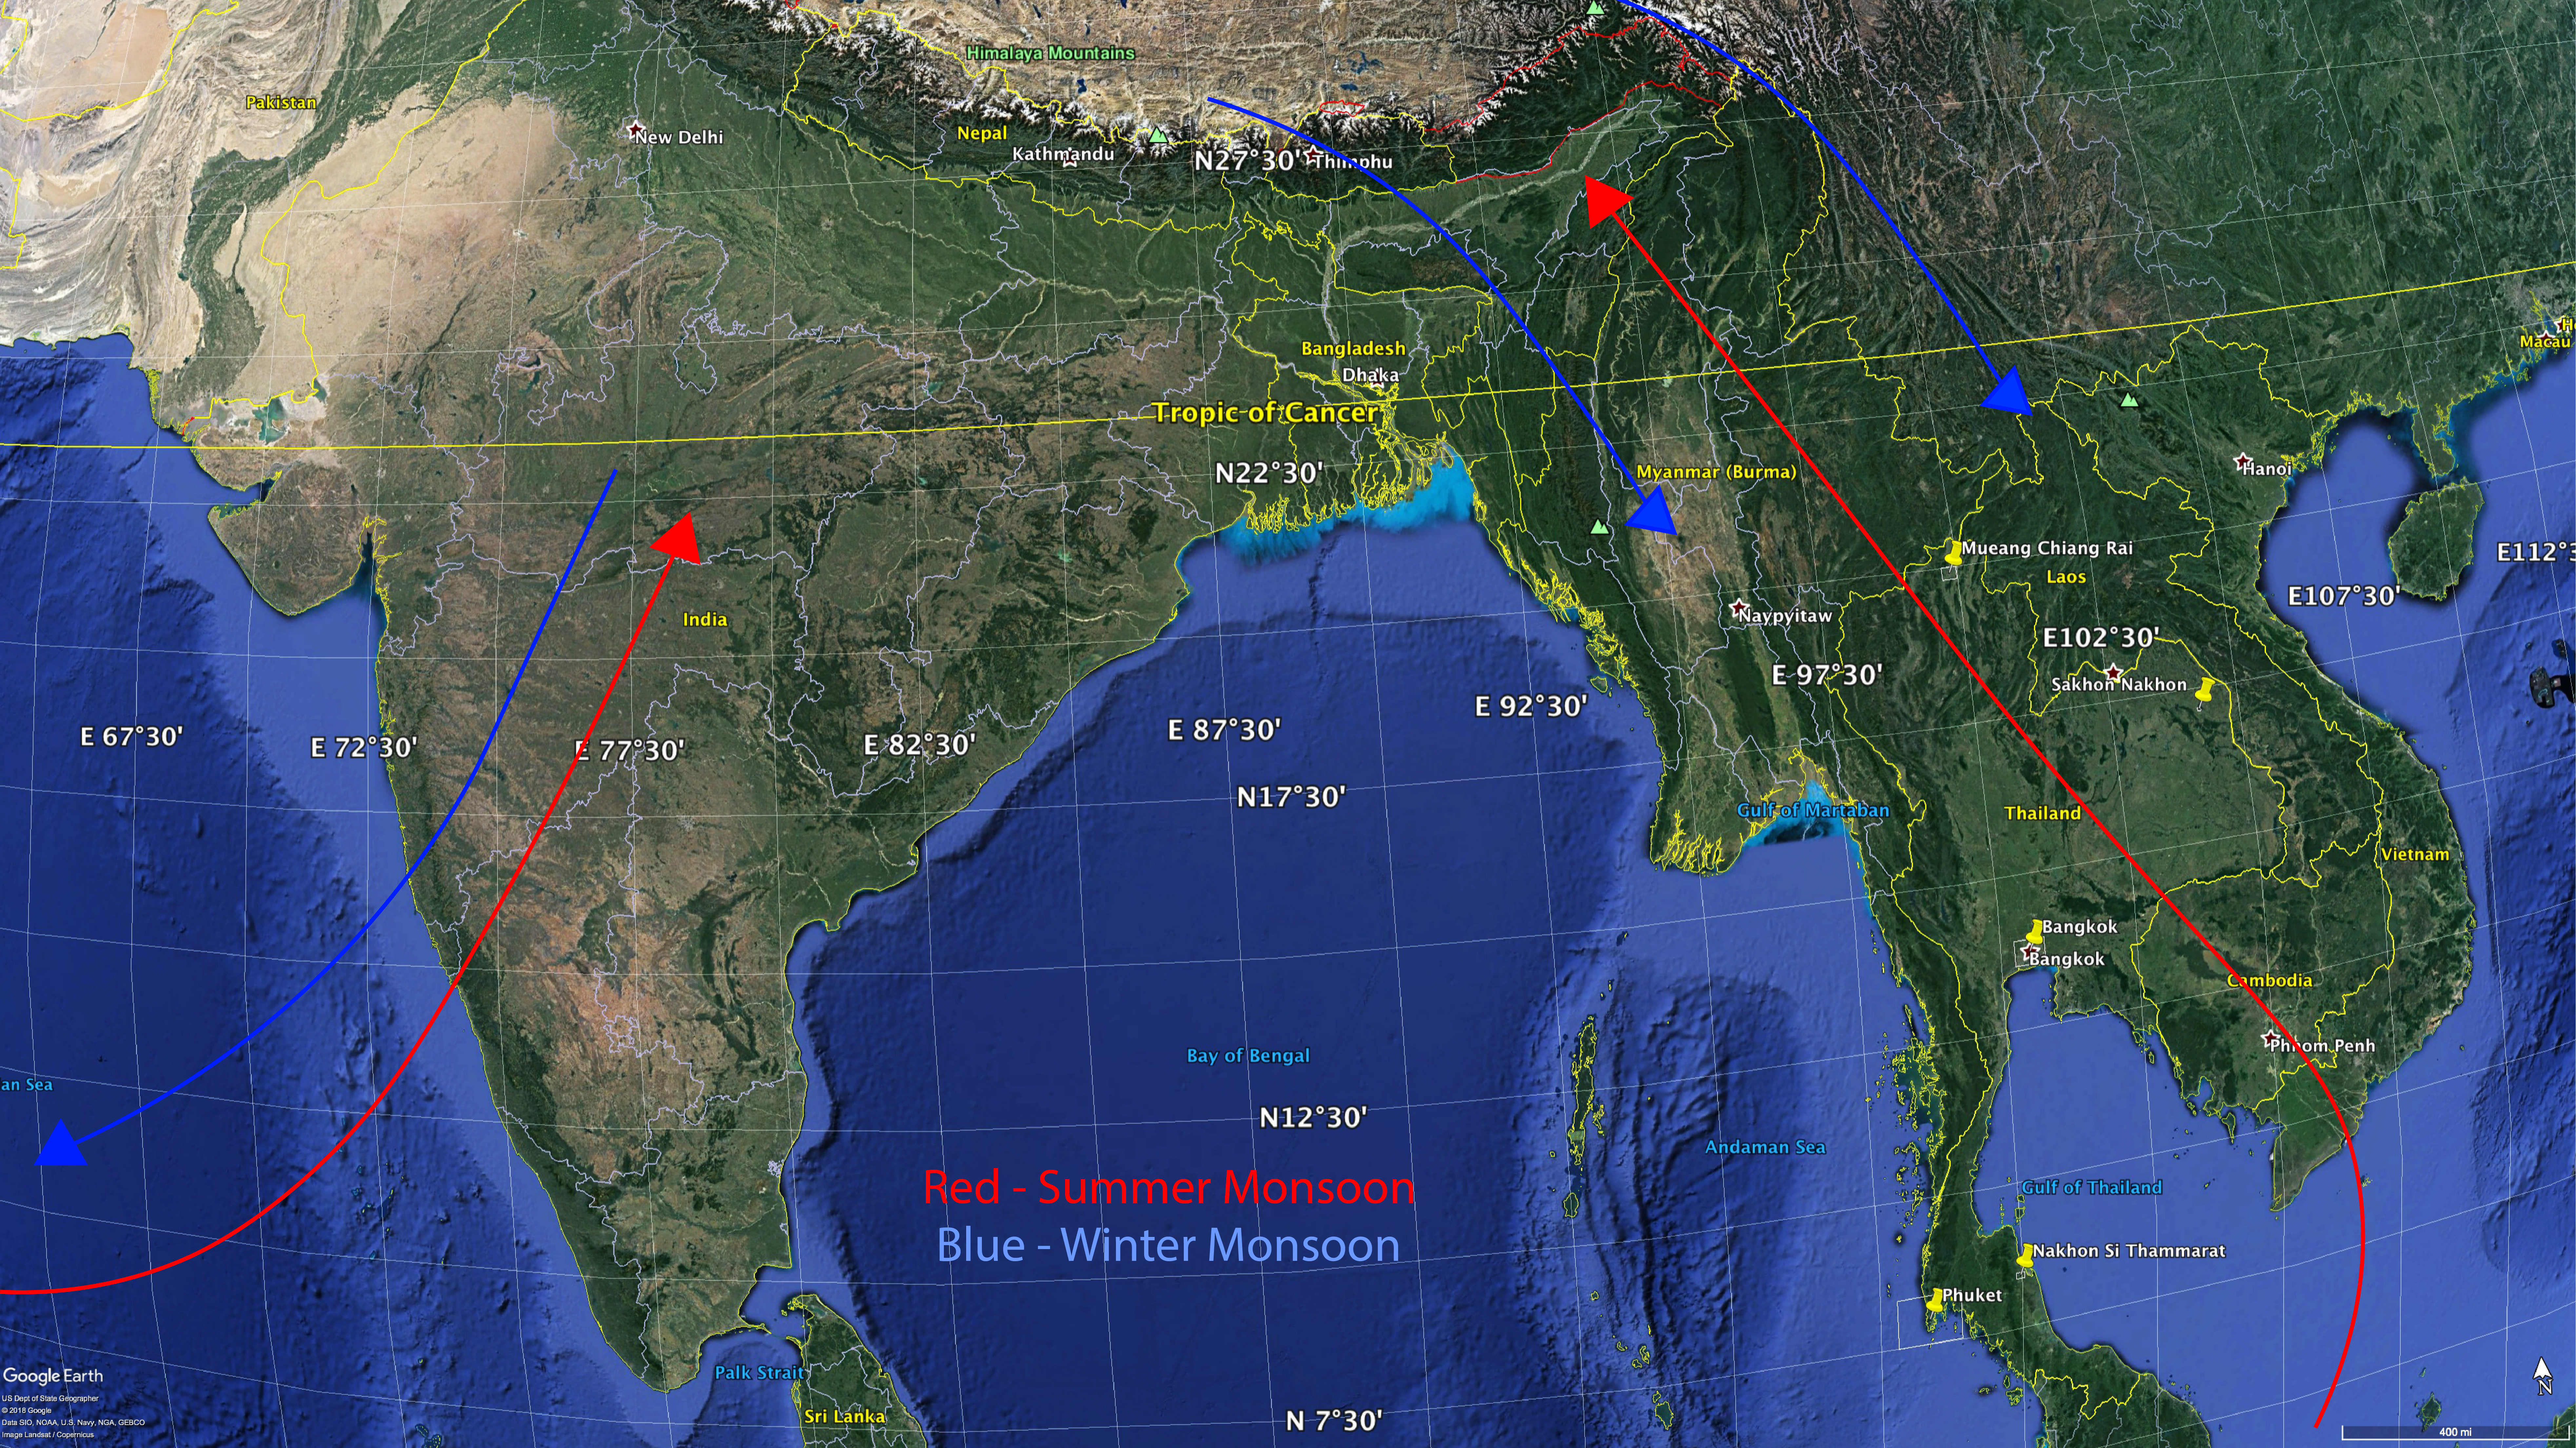
\includegraphics[width=\linewidth]{AsianMonsoon}
  \caption{The cycle of summer and winter moonsons in Asia. In the figure, the arrows represent moisture-laden winds.}
  \label{fig:asianmonsoon}
\end{figure}
 
\subsubsection{Impacts of Monsoons}

Billions of people around the globe depend on Monsoon rains for their yearly rainfall. For example, farmers in Myanmar�s Rakhine state need the rainfall from the Wet Monsoon season to cultivate paddy rice, especially since the Summer Monsoon brings in 80\% of the subcontinents rainfall. As agriculture contributes to 37.8\% of Myanmar�s economy, the arrival of the Monsoon season is crucial to the livelihoods of many citizens of Myanmar \citep{monsoonimpact}.

However, intense rainfall in these regions can cause massive flooding and mudslides, destruction of crops, and kill hundreds of people in floods. For example, during extreme Monsoon weather in Myanmar in 2015,  more than 1.4 million acres of farmland was flooded. Twelve out of the country's 14 provinces were affected, with northern and western regions suffering the hardest blows.385,000 households have been displaced by the floods, and landslides have destroyed thousands of homes \citep{monsoonimpact}.

\subsubsection{Monsoons in the future}
According to the IPCC, all models and all scenarios project an increase in both the mean and extreme precipitation in the Summer Monsoon. This could lead to major flooding events, especially in Southeast Asia.\citep{monsoonfuture}

\subsubsection{Effect of Monsoons on typhoons}
Typhoons normally occur during the same time as the Summer Monsoons, as they are strongest between the months of June through November in Southeast Asia. Wind pulls moisture from the warm oceans, and as the moisture floats upwards it is converted into warm air and heat. The heat causes more air to flow to the center of the storm, causing evaporation. Finally, all of the heat and air flow towards the eye, creating a typhoon. Due to warming seas, the destructive power of the typhoons that wreak havoc across Indonesia and the Philippines has intensified by 50\% in the past 40 years. Researchers warn that global warming will lead giant storms to become even stronger in the future, threatening the large and growing coastal populations of those nations. Typhoons can have devastating impacts in east Asia. In 2013, typhoon Haiyan hit the Philippines, killing at least 6,300 people and affecting 11 million \citep{typhoon}.

\subsubsection{Chapter Exercise: Monsoons}
Now that you know something about Monsoons, try drawing a diagram to demonstrate the difference between the Summer and the Winter Monsoon. Print out a map of South East Asia and add arrows to the map to show the different directions that te wind will move in!

\subsubsection{El Ni\~no-Southern Oscillation (ENSO) cycle}

The ENSO cycle is a scientific term that describes the fluctuations in temperature between the ocean and atmosphere in the east-central Equatorial Pacific area. The cycle is a natural phenomenon and includes El Ni\~no and La Nina, with both processes occurring from December to February \citep{enso}. 

\begin{figure}[h!]
  \includegraphics[width=\linewidth]{ENSO}
  \caption{The El Ni�o Cycle. Figure via the Climate Prediction Center of the NOAA National Centers for Environmental Prediction.}
  \label{fig:ENSO}
\end{figure}

\subsubsection{What is El Ni\~no}
El Ni\~no occurs every three to five years and begins when warm water in the western tropical Pacific Ocean shifts eastward along the equator toward the coast of South America. Normally, this warm water pools near Indonesia and the Philippines. However, during an El Ni\~no, the Pacific's warmest surface waters sit offshore of northwestern South America. This leads to Southeast Asia�s hot and dry climate, which usually occurs around the month of April, as the moisture is shifted towards South America \citep{enso}. 

\subsubsection{Effects of El Ni\~no}

One of the strongest El Ni\~no event in Southeast Asia happened in 1997. Then, fires, fueled by a drier rainy season in many parts of Indonesia, burned an estimated 5 million hectares, creating a haze that affected most of the region. The dry weather also caused massive food shortages in Indonesia, causing the government to import 5.8 million tons of rice due to drought and fire-related crop failures. Looking at the model predictions for the next 50 years, the researchers found that the impact of climate change could amplify the effects of each El Ni\~no, leading to temperature records being broken more often. However, researchers also mentioned that preparedness could allow societies in this region to cope with climate change. Since El Ni\~no can potentially be predicted a few months in advance, this could help societies prepare for extreme drought \citep{elninoindo}. 

\subsubsection{What is La Nina}
La Nina is the cooling of sea surface temperatures in the eastern and central Pacific. In general, this triggers wetter weather in South-East Asia and parts of Australia. Unusually strong, eastward-moving trade winds and ocean currents bring cold water to the surface east of the pacific ocean, a process known as upwelling. This leads to high air pressure in the east pacific, leading the air to flow to the western pacific, where the air pressure is lower and the temperatures are higher. These low-pressure zones contribute to increased rainfall in Southeast Asia \citep{enso}. 

\begin{figure}[h!]
  \includegraphics[width=\linewidth]{JakartaFloods}
  \caption{Flooding in Jakarta, Indonesia}
  \label{fig:jakartafloods}
\end{figure}

\subsubsection{Effects of La Nina}
Persistent heavy rains from La Nina led to flooding and landslides throughout Indonesia in late December 2007 and early January 2008, resulting in numerous fatalities and crop losses. The most heavily populated island in the chain, Java, was the hardest hit, and at least 112 people died on the island from flooding or landslides. \citep{elninoindo}.

\subsection{Is the weather a boring topic?}

Oscar Wilde wrote.... there is nothing so boring as the weather... It this true?


As in the case of flooding in Thailand, good meteorlogical data has the potential to save lives. Since 1980, the number of natural disasters in the world and the number of people affected has risen. However, thanks to effective forecasting, the number of people killed has not risen. Today, an increasing number of people are situated in regions of high risk for weather hazards. Developing countries are going to be exposed to more extreme weather events due to climate change. The world�s population is exploding, city populations are exploding and weather/climate related diseases are now killing a million people every year. Most of the people are killed are children under the age of 5 in developing countries. Weather and climate forecasting is essential to combat all these problems \citep{preparedness}.For instance, weather forecasting was used to predict Typhoon Bopha in the Philippines in 2012, which helped mitigate a climate disaster. Through forecasting, Filipino citizens had information to wind speed, location of incoming weather disturbances, and possible amounts of precipitation. By predicting the Typhoon, the early warning Typhoon systems helped evacuate 167,000 people to shelters. Forecasting will continue to be incredibly important for this region in the future, as the IPCC predicts that that climate change is likely to cause tropical cyclones to become more severe with greater wind speeds and more intense precipitation.\citep{typhoon} 

In addition to the fact that effective meteorological systems can help save lives through effective hazard forecasting, they also have considerable economic benefits. These benefits result from the improved economic decisions that stakeholders can make with the knowledge that comes from meteorology. For instance, sound climatological meteorological information can help farmers make decisions about what crops to grow and when to grow them. It can help the energy industry in optimizing the generation, transmission and distribution of power. All in all, hydrometeorological information has significant impacts in the management of road traffic, railway traffic, the maritime industry, aviation, construction, energy, air quality and agriculture. A Swiss study found that that the cost-to-benefit ratio of meteorological services is likely between 1:4 and 1:6 \citep{swissmeteo}. A Chinese study found that the value of the benefit of the Chinese Public Weather Service was at least 46 billion Chinese Yuan in 2006 \citep{chineseservice}. 




 

\subsection{The Dynamic Climate System}
According to the IPCC, mean annual temperature is likely to have increased over the past century over most of the Asian region. Furthermore, it is likely that the numbers of cold days and nights have decreased and the numbers of warm days and nights have increased across most of Asia since about 1950 \citep{ipcc}.For this section, we will be analyzing trends in increasing rainfall and temperature in two countries in Asia: Thailand and Singapore. This was achieved by downloading the climate data from NOAA, and using the data to evaluate to evaluate long term climate patterns for these two countries. 

Singapore is affected by increasing temperatures, as from 1972 to 2014, the annual mean temperature has increased from 26.6�C to 27.7�C. As Singapore is an island, data was downloaded from the only weather station with data on temperature and precipitation.\citep{singaporeclimatechange}

Thailand is also affected by rising temperatures, and Average annualtemperatures have significantly risen by about 0.95� C between 1955 and 2009. Thailand has 53 weather stations, and so five stations were picked in different areas of the country for an overall climate assessment of the country. For  both Thailand and Singapore, data was first collected from 1950 until the present day. 

\subsubsection{Why were Singapore and Thailand chosen?}
Singapore and Thailand were chosen because both countries differ geographically and economically, yet are in close proximity to each other. Thailand is much larger than Singapore, and has a size of 513,120 km�, compared to Singapore�s 719.9 km�. Due to Thailand�s large size, it is split up into 76 provinces, with most of the development and economic resources concentrated in the capital, Bangkok. However, Singapore is a island, and so the development and economic resources are mostly tantamount for the entire country. Both countries are found near the equator and are 945 km away from each other, and so the climate for Singapore and Thailand, especially Southern Thailand, should be similar to each other. By analyzing these two countries, climate and rainfall can be compared between a small developed and a large developing country.

\subsubsection{Which areas were chosen within each country?}

As Singapore is a small island with one weather station, that station was chosen. 

However, five geographically different locations with different degrees of development in Thailand were chosen in order to get an accurate representation of weather in the country. Bangkok (a urban area in the center), Chiang Rai (a urban-rural area in the North West), Sakon Nakhon (a rural area in the North East), Phuket (a urban area in the South West), and Nakon Si Thammarat (a urban-rural area in the South East) were chosen. These stations are illustrated in Figure \ref{fig:stationsmap}

\subsubsection{What months were picked?}

For Singapore, January, May, and November were selected. These months were chosen because January is the coldest month, May is the hottest month, and November is the rainiest month \citep{singaporeweather}. 

For Thailand, January, April, August were selected. These months were chosen because January is the coldest month, April is the hottest month, and August is the rainiest month \citep{thailandweather}. 

\begin{figure}
  \includegraphics[width=\linewidth]{ClimateMapEnhanced}
  \caption{The NOAA stations in Thailand chosen for analysis in this chapter. They are depicted on top of a raster which shows the prevailing average temperatures and humidity in Thailand in May. This is to help indicate why these particular NOAA stations were chosen.}
  \label{fig:stationsmap}
\end{figure}

\section{Climate Data}

\subsection{What is graphed?}
A linear regression of Monthly Average Rainfall and Maximum Temperature are graphed below. Monthly Average Rainfall can analyze changes in precipitation, and Maximum Temperature can attest to change in temperature. Maximum temperature is chosen over average temprature because there is not a strong enough trend for average temperaure. Reasons for this are not apparent, and more reserach should be done on this subject.  

\subsection{Overall Temperature Trend}
From 1880, global surface temperature has increased 0.07�C every 10 years. However, the past century has seen a warming of 0.74�C. \citep{tempincrease}. Both Thailand and Singapore have seen an increase in maximum temperature.

\subsubsection{Singapore}
Major climate models show that Singapore has warmed gradually by about 0.25 deg C in each decade from 1948 to 2015, and that temperatures will continue to increase. In our temperature analysis, we found out that Singapore's maximum temperature has been increasing from 1950 to the present day for the months of May, November, and January. For all three months, there are positive upwards trend line and statistically significant results. The p-value for all three months is less than 0.05, and thus statistically significant. \citep{singaporeweather}

\begin{figure}[h!]
\centering
  \includegraphics[width=.8\linewidth]{TMAX_Singapore}
  \caption{Average Monthly Maximum Temperature in Singapore}
  \label{fig:TMAX_Singapore}
\end{figure}

\subsubsection{Thailand}

Major climate models indicate a temperature rise for the whole country of Thailand, particularly the central plain and lower North-eastern region. However, there is no specific literature analysing the picked regions. Projections show that mean temperatures in central Thailand, including Bangkok, has been increasing by 0.4 in each decade from 1958 to 2014. In our temperature analysis, we found that Thailand's maximum temperature is increasing overall for all five locations, however, not every month is statistically significant. On the other hand, Bangkok seems to show a significant trend which is congruent with the predictions that central Thailand�s temperature will be increasing.  \citep{bkkweather}

\textbf{Bangkok}: Bangkok's maximum temperature has been increasing from 1950 to the present day for the months of April, August, and January. All three months have steep upward positive trend lines, and all three months are statistically significant, as the p value for all months is lower than 0.05.

\begin{figure}[h!]
  \centering
  \includegraphics[width=.8\linewidth]{TMAX_Bangkok}
  \caption{Average Monthly Maximum Temperature in Bangkok}
  \label{fig:TMAX_bangkok}
\end{figure}

%\textbf{Chiang Rai}: Chiang Rai's maximum temperature has been increasing from 1950 to the present day for the months of August and January. Both of these months have steep upward positive trend lines, and are statistically significant, as the p value for both months is lower than 0.05. April has a downards gentle negative line trend, showing a decrease in maximum temperature. However, the p value is 0.326, larger than 0.05, and so this result is not statistically significant. 





%\textbf{Sakon Nakhon}: Sakon Nakhon's maximum temperatu%re has been increasing from 1950 to hte present day for %the month of August. There is a steep positive trend %line with a statistically significant p value lower %than 0.05. However, the months of January and April %have a horizontal trend line, with p values of 0.96 and 0.99, very statistically insignificant.

%\begin{figure}[h!]
%  \centering
%  \includegraphics[width=.8\linewidth]{TMAX_Sakon}
%  \caption{?? in Sakon}
%  \label{fig:TMAX_Sakon}
%\end{figure}


%\textbf{Nakon Si Thammarat}:Nakon Si Thammarat's maximum temperature has been increasing from 1950 to the present day for the months of April, August, and January. January and August have steep upward positive trend lines, with statistically significant p values lower than 0.05. However, April, which has a positive upward trend line, has a pvalue of 0.127, which is statistically insignificant.  

%\begin{figure}[h!]
%  \centering
 % \includegraphics[width=.8\linewidth]{TMAX_Nakon}
%  \caption{?? in Nakon}
%  \label{fig:TMAX_Nakon}
%\end{figure}

%\textbf{Phuket}: Phuket's maximum temperature has been increasing from 1950 to the present day for the months of April, August, and January. All three months have steep upward positive trend lines, and all three months are statistically significant, as the p value for all months is lower than 0.05. 

%\begin{figure}[h!]
%\centering
%  \includegraphics[width=.8\linewidth]{TMAX_Phuket}
 % \caption{?? in Phuket}
%  \label{fig:TMAX_Phuket}
%\end{figure}

\subsection{Overall Rainfall Trend}
According to the IPCC, the annual total wet-day rainfall in South East Asia has increased by 22 mm per decade, while rainfall from extreme rain days has increased by 10 mm per decade. Furthermore, between 1955 and 2005 the ratio of rainfall in the wet to the dry seasons increased, and there has been an increasing in frequency of extreme rainfall events in the northern parts of Southeast Asia \citep{REF}.

\subsubsection{Singapore}
Rainfall in Singapore has become more intense in recent years. According to Singapore's Second National Climate Change Study, there has been a general uptrend in annual average rainfall from 2192mm in 1980 to 2727mm in 2014 \citep{singaporeclimatechange}. In our rainfall analysis, we found out that  Singapore's monthly average rainfall has been increasing from 1950 to the present day for the months of May, November, and January. For all three months, there is a positive upwards trend line and statistically significant results. The p value for all three months is less than 0.05, and thus statistically significant.   

\begin{figure}[h!]
\centering
  \includegraphics[width=.8\linewidth]{PRCP_Singapore}
  \caption{Monthly Average Rainfall in Singapore}
  \label{fig:PCRP_singapore}
\end{figure}


\subsubsection{Thailand} 
There has been no significant change of rainfall volume in Thailand, and the total amount of rainfall between 1955 and 2014 did not change significantly. However, there has been evidence that there has been increasing rainfall in the Northeast and Gulf region as well as the Bangkok area. \citep{bkkweather}. In our rainfall analysis, there is no clear trend for Thailand�s monthly average rainfall. For some areas, rainfall is increasing, and for some areas rainfall is decreasing. However, Bangkok's monthly average rainfall is increasing. 

\textbf{Bangkok}: Bangkok's monthly average rainfall has been increasing from 1950 to the present day for the months of August and January. Both these months have steep upward positive trend lines, and are statistically significant, as the p values are lower than 0.05. However, August which has a downward negative trend line, has a p value larger than 0.05, which is statistically insignificant. 

\begin{figure}[h!]
  \centering
  \includegraphics[width=.8\linewidth]{PRCP_Bangkok}
  \caption{Monthly Average rainfall in Bangkok}
  \label{fig:PRCP_bangkok}
\end{figure}

%\textbf{Chiang Rai}: Chiang Rai's monthly average rainfall has been increasing from 1950 to the present day for the months of April and January, but decreasing for August. However, the p values for all three months are larger than 0.05, proving the results to be statistically insignificant. 

%\begin{figure}[h!]
 % \centering
  %\includegraphics[width=.8\linewidth]{PRCP_Chaingrai}
 % \caption{?? in Chaingrai}
  %\label{fig:PCRP_chaingrai}
%\end{figure}

%\textbf{Sakon Nakhon}: Sakon Nakhon's monthly average rainfall has been increasing from 1950 to hte present day for the months of August, April, and January. While all three curves for slope upwards, the gradient is rather gentle. Furthermore, the p values for all three curves are larger than 0.05, deeming the results as insignificant.

%\begin{figure}[h!]
 %\centering
  %\includegraphics[width=0.8\linewidth]{PRCP_Sakon}
  %\caption{?? in Sakon}
  %\label{fig:PCRP_Sakon}
%\end{figure}

%\textbf{Nakon Si Thammarat}:Nakon Si Thammarat's monthly average rainfall has been increasing from 1950 to the present day for the months of April, August, and January. January has a steep postive upward trend line, and has a p value lower than 0.05, a statistically significant result. August and April both have an upward positive curve. However, the p values for both curves are larger than 0.05, a statistically insignificant result.  

%\begin{figure}[h!]
%\centering
 % \includegraphics[width=.8\linewidth]{PRCP_Nakon}
%  \caption{?? in Nakon}
 % \label{fig:PRCP_Nakon}
%\end{figure}

%\textbf{Phuket}: Phuket's monthly average rainfall has been increasing from 1950 to the present day for the months of August, and January. August has a steep upward curve with a p value smaller than 0.05, the result is statistically significant. However, January, while an increasing curve, has a p value larger than 0.05, a statistically insignificant result. April's curve is decreasing, however, the p value is larger than 0.05, a statistically insignificant result. 

%\begin{figure}[h!]
%\centering
 % \includegraphics[width=.8\linewidth]{PRCP_Phuket}
%  \caption{Monthly Average Rainfall in Phuket}
 % \label{fig:PCRP_Phuket}
%\end{figure}

\begin{exercise}
Temperature and rainfall graphs

Now that you know what temperature and rainfall graphs look like, pick your own region and download data for it from NOAA $($https://www.ncdc.noaa.gov/cdo-web/$)$. Make your own temperature or rainfall graph! Does it agree with the temperature and rainfall trends of Bangkok and Singapore?
\end{exercise}


\subsection{Why are temperatures rising in Bangkok and Singapore?}



\subsubsection{The Urban Heat Island Effect}
The Urban Heat effect occurs when heat and air temperature in densely built urban areas are higher than in the surrounding areas. This occurs when there is a lack of vegetation and soil moisture, which would normally be used to absorb the sunlight to evaporate water through photosynthesis. The heat that is absorbed during the day through buildings, roads, and other types of construction is reemitted during the night. The heat's energy contributes to raising the temperature of the surfaces and air around the urban areas. Furthermore, buildings can block wind, a cooling factor, which further leads to higher temperatures in cities. \citep{urbanheatisland}.  

Singapore has shown to be affected by the urban heat island effect, as shown in our graph by the steep increase in maximum temperature. According to a study published by the National University of Singapore, the high rise central district has a  2�C higher temperature at night compared to other areas with low-rise buildings. As the maximum temperature graph shows, maximum temperature in Singapore has been steeply increasing,  \citep{{singaporeclimatechange}}. 

Bangkok, the most developed and urban area in Thailand, is also affected by the urban heat island effect, as shown in our graph by the steep increase in maximum temperature. According to a study published by Istanbul University, Bangkok has  a 0.8�C higher temperature than the surrounding states of Bangkok \citep{bkkweather}. 

\subsubsection{Chapter Exercise: The Urban Heat Island Effect}
On a map, mark the cities, suburbs, rural areas and water bodies in the region where you live. Using the internet, find the average temperatures for these places in any given month and add this information to your map. Can you see the urban heat island in effect, as in Figure \ref{fig:urbanheat}?.

\begin{figure}[h!]
  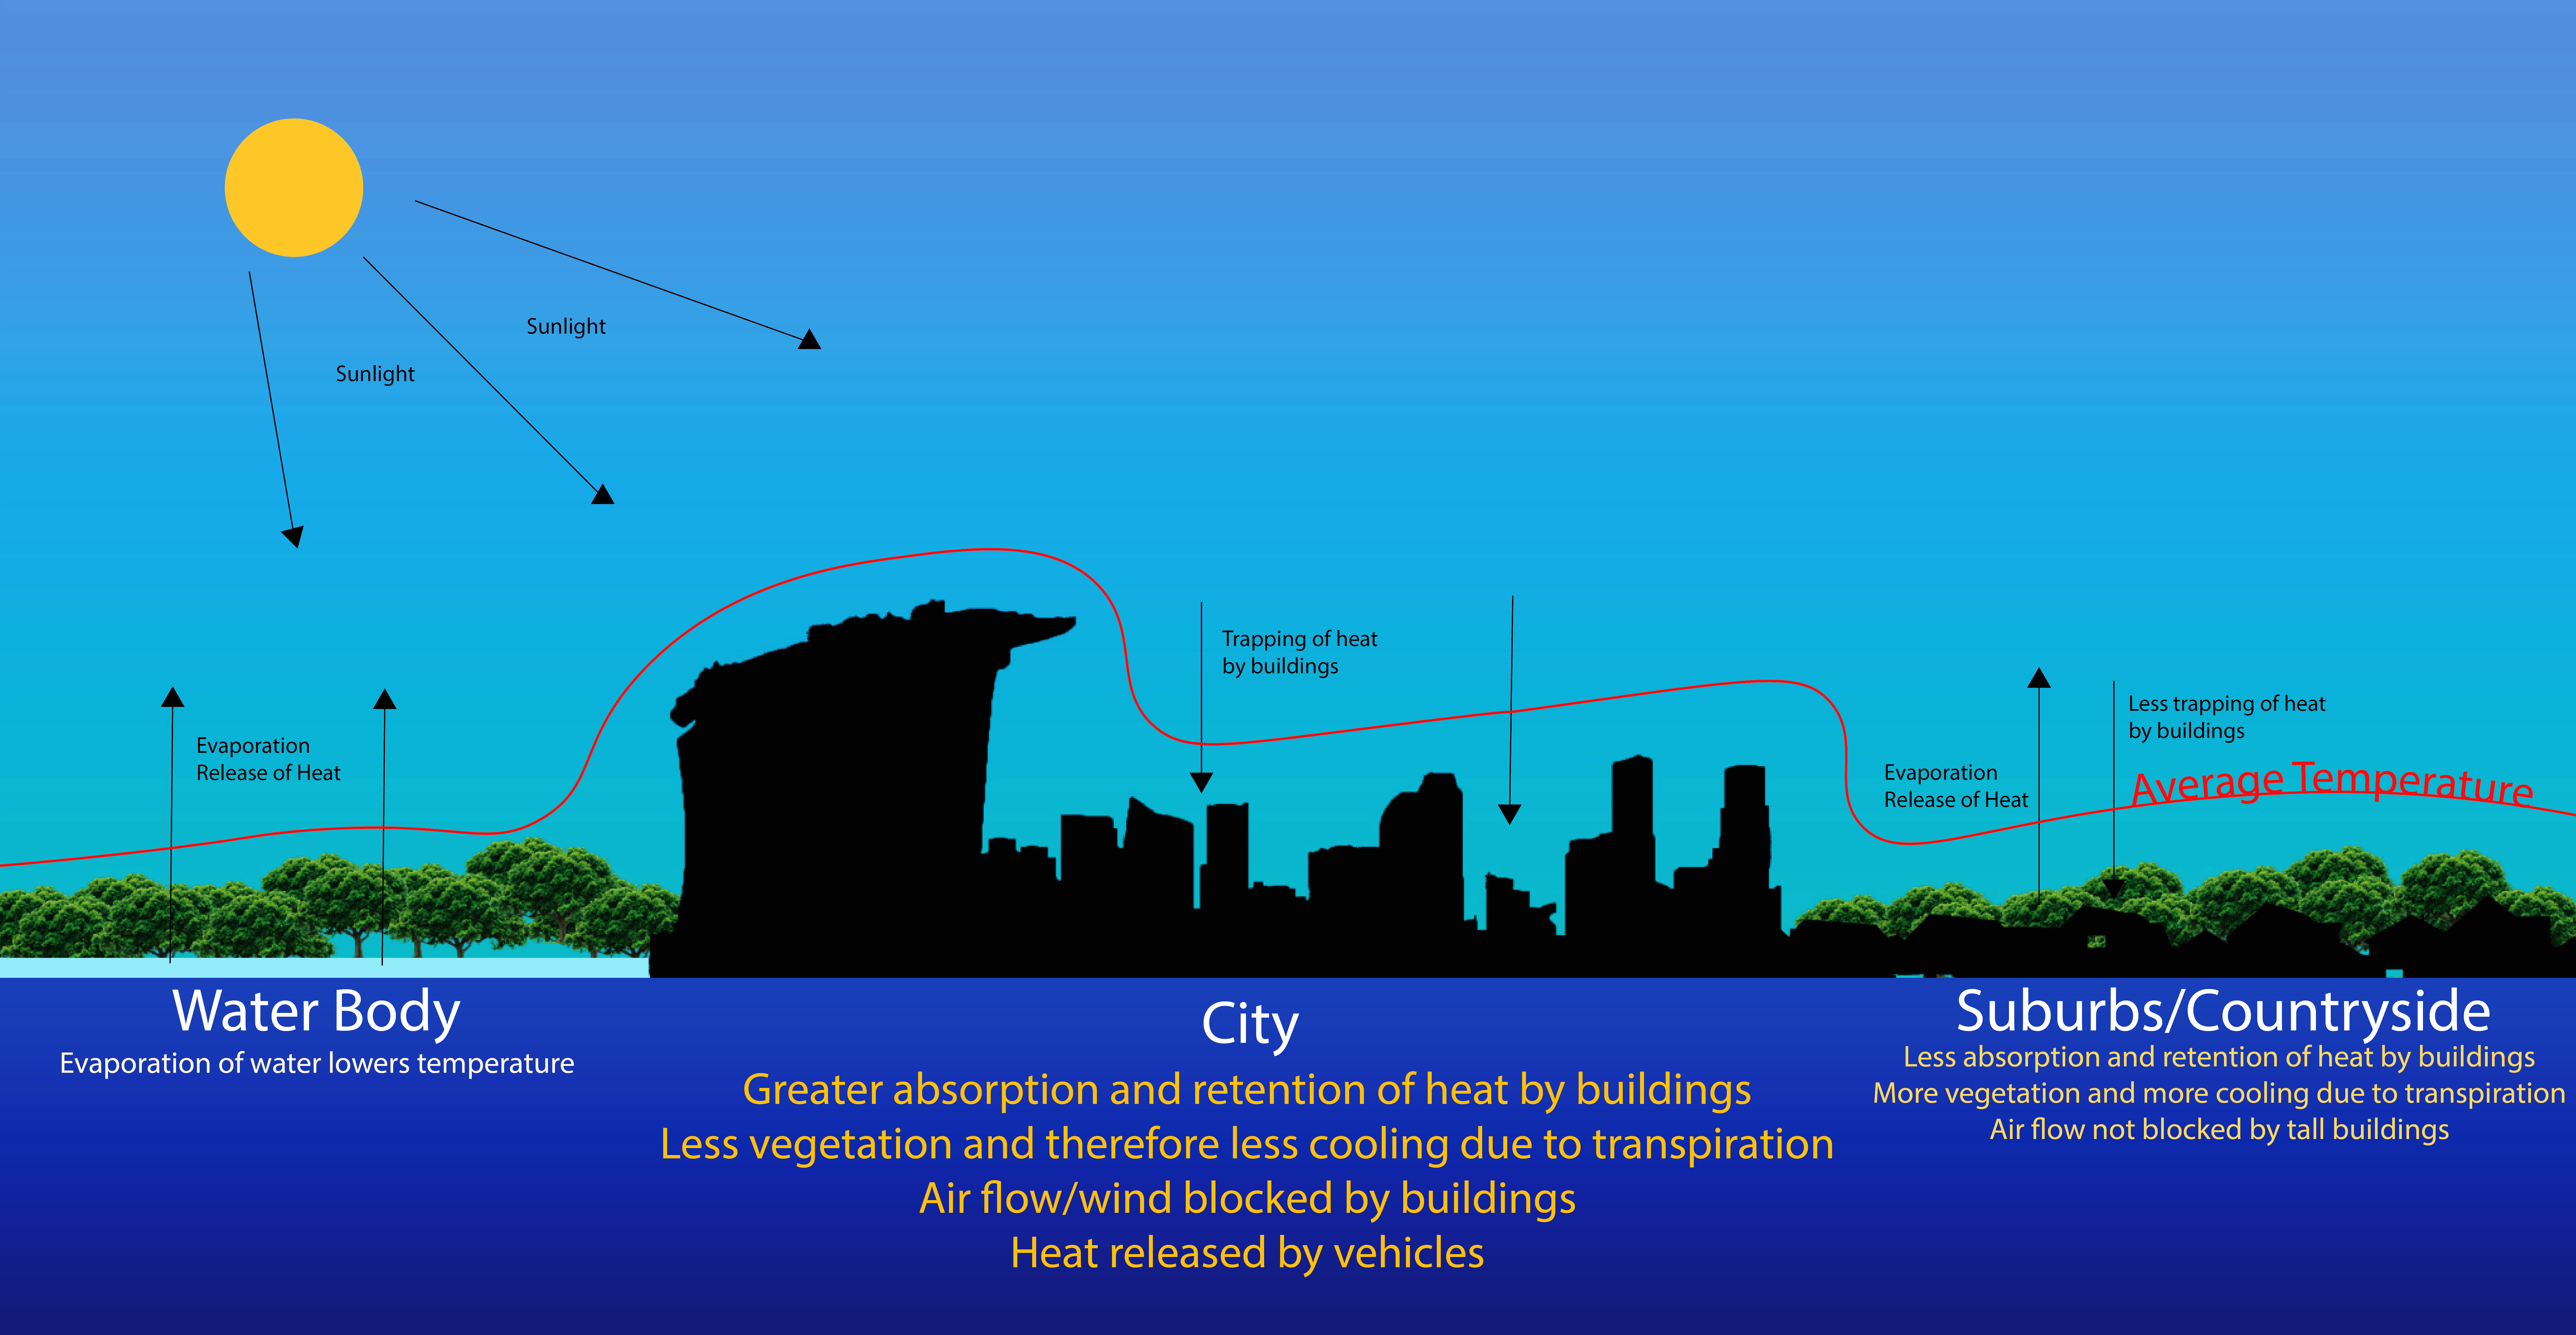
\includegraphics[width=\linewidth]{UrbanHeatIslandEnhanced}
  \caption{The Urban Heat Island Effect}
  \label{fig:urbanheat}
\end{figure}

\subsection{Does the observed variability have anything to do with human forcing?}

In recent times, increasing awareness of the phenomenon of anthropogenic climate change has led to an increased effort to examine the role of human forcing in observed weather conditions and long-term climate trends. Greenhouse gas forcing has been tied to the patterns of anomalously high rainfall in the pre-Monsoon season leading up to the great flood of 2011 in Thailand, and thus these greenhouse gas emissions functioned as one of the forcing mechanisms for the flood itself \citep{floodfailure}. 

\section{What are the socio-economic implications for the countries analyzed?}

Our climate affects everything around us, including vital life indices. As long term climate change trends are being uncovered in meteorological data, a large number of studies are being published on the impact of these changes on essential factors such as food availability, the spread of diseases, water access and infrastructure. 

\subsection{Healthcare}
In Thailand, the occurence of liver fluke exhibits a strong positive correlation with precipitation and temperature, two factors which are being impacted by climate change \citep{liverfluke}. Temperatures in Thailand are clearly rising, as shown in Figure \ref{fig:TMAX_bangkok}, and the patterns of precipitation in the country are changing, as shown in Figure \ref{fig:PRCP_bangkok}. It is likely that liver fluke may exacerbated by ongoing climate changes.

In Singapore, the number of dengue cases was found to be correlated with temperature, but no statistically significant relationship was found with precipitation or humidity \citep{singaporedengue}. Temperatures in Singapore are also clearly rising, as shown in Figure \ref{fig:TMAX_Singapore} which means the number of dengue cases is forecasted to increase as well.

The comparision of Singapore to Thailand here can also be thought of in terms of their relative wealth. Singapore is situated in a region where vector-born diseases like dengue are endemic. However, because it is wealthy, the effects of climate change have not caused too many public health problems there. In fact, Singapore is the country which has made the most progress towards achieving health related UN Sustainability Goals \citep{sinagaporeclimatechange}. Thailand, on the other hand, is developing nation. It is much more prone to the occurence of a public health crisis through increased occurence of both insect-borne and water-borne diseases. In fact, the World Health Organization predicts that over 70 million people in Thailand will be at a signficant risk of contracting malaria \citep{borgen}.

\subsection{Water access}

Singapore is widely known as a country with a water scarcity problem. Climate change is expected to create significant sea level rise and temperature increase in Singapore by 2100, which will further stress the country's water resources, and have led it to establish a National Climate Chage Committee, which has enacted policies to protect the country from coastal erosion, flooding and loss of vital water supply \citep{bhullar2013climate}. 

Thailand does not have as much of a water scarcity problem, but significant degradation of forests and projected land use changes in the near future, combined with projected decreases in rainfall, are expected to decrease the yield and increase the sediment load of the Thadee watershed, a major source of water for agriculture and household use in the Nakhon Srithammarat Province in Southern Thailand \citep{landuse}. 

\begin{figure}
  \includegraphics[width=\linewidth]{singaporepipe}
  \caption{The water pipeline at the Johor-Woodlands Causeway which brings 54\% of Singapore's water supply from Malaysia\citep{shaaz2008}}
  \label{fig:waterpipe}
\end{figure}

\subsection{Food}
An analysis of the climate indices that most affect rice production in Southeast Asia, specifically the onset of the wet season and nighttime temperatures, found that over the period from 1971-2012, nighttime temperatures were found to have increased, as shown in Figure \ref{fig:TMAX_bangkok}, which has had an adverse effect on rice yields \citep{riceindices}. 

Poorer farmers are especially vulnerable to changing climate. An economic analysis of the impact of climate change on rice yields in Thailand which integrates soil science crop modeling, weather simulators, and global climate change modeling found that �overall, farmers are unable to neutralize the adverse effects of the more extreme climate change. However, they are able to cope with milder climate change and even benefit slightly from small increases in rainfall. While most farmers manage to adjust to milder climate change, poor farmers are less able to do so" \citep{climatechangerice}. Farmers' perceptions of changes in temperature and precipitation are generally consistent with the trends seen in Figures \ref{fig:TMAX_Singapore} and \ref{fig:PRCP_bangkok}. Agricultural experiences, farm income, training, social capital, and effective climate adaptation communication are all significant factors in increasing the probability of them adapting to these climate changes \citep{farmerintention}.

The mountains of Northeast Thailand mostly see farming of low-value crops, which can be grown equally well in the lowlands. A study found that these mountains have a distinct advantage for the production of high-value fruits and vegetables, and planting of these high value crops represents a significant opportunity for agricultural development \citep{mountains}.  However, these fruits and vegetables are suited for temperate climates, and the potential for their cultivation may be impacted by the warming trend shown in figure \ref{fig:TMAX_bangkok}. 

Singapore, unlike Thailand, is not an agricultural hotspot. It imports over 90\% of its food , which makes it particularly vulnerable to fluctuations in global food supply and prices \citep{singaporeclimatechange}. 

\subsection{Biodiversity}

Changes in climatic conditions are having a massive impact on biodiversity all over the world. Because species evolve over long periods of time to live within certain range sof temperature, it is projected that by 2050,  25\% of all species will become extinct just because of rapid, anthropogenically induced climate change \citep{harvardbio}. 

Many species have responded to climate change by shifting their habitation ranges polewards, to avoid the warmer temperatures developing in pervading their original habitats. In Thailand, protected areas, which are on average 2�C cooler than the surrounding regions, are becoming increasingly vital for conservation of organisms such as tropical butterflies. Their importance is being further accentuated by the fact that most protected areas in Thailand are located at higher elevations, making them well suited to become habitats for species of butterflies migrating from lower elevations \citep{butterflies}. 

Biodiversity conservation measures in Southeast Asia may be impeded by a lack of willingness on the part of the local populations. For instance, a study conducted in households in China, Vietnam, the Philippines and Thailand found that people place a low priority on the conservation of animals such as marine turtles, and would be unwilling to accept additional taxes for conservation measures. This is likely a result of the fact that per-capita incomes in the region are generally not as high as in Western nations, and people do not trust government expenditure systems. This makes biodiversity conservation in the region something that may require international, rather than just local attention \citep{turtles}. 

For more on biodiversity and climate change, see \textbf{Chapter 6: Biomass}. 

\subsection{Air Quality}
Air quality is closely related to meteorological factors such wind speed, humidity, temperature, rainfall and solar radiation.  In Singapore, air quality standards have generally met the standards of the United States Environmental Protection Agency $($EPA$)$ and the World Health Organization $($WHO$)$ \citep{singaporeaq}. However, it is affected by the Southeast Asian Haze, which results from the slash and burn practices prevalent in the forests of Indonesia. This haze can make the air in Singapore dangerous to breathe. Understanding and combating this haze requires us to look into aerosol transport in the region using weather research and forecasting models \citep{singahaze}. The El Nino climate phenomenon described in \ref{fig:ENSO} can create exceptionally dry conditions in Indonesia, which can exacerbate forest fires there, and, by extension, the haze \citep{bbchaze}.   
For more on the Southeast Asian Haze, consider reading \textbf{Chapter 7: Peatlands}. 

\begin{figure}
  \includegraphics[width=\linewidth]{seasiahaze}
  \caption{A NASA satellite image of forest fires over Indonesia, which cause the Southeast Asian Haze \citep{bbchaze}}
  \label{fig:seaasiahaze}
\end{figure}

In Bangkok, a study has shown that there is a positive correlation between the trend of increasing temperatures seen in Figure \ref{fig:TMAX_bangkok} and PM2.5 concentrations. The city's air quality is already below the standards set by Thailand's Pollution Control Department, so climate change is exacerbating the problem. These increased PM2.5 concentrations are correlated with increased occurences of respiratory and circulatory diseases \citep{airpolchapter}. 

\subsection{Infrastructure}

The dual challenge of both mitigating and adapting to the effects of climate change are significant ones. Policymakers and scientists need to seek inspiration from a variety of sources to design effective solutions. Incorporation of local and indigenous knowledge into climate change mitigation strategies is essential for this purpose. 

For instance, small island communities in Indonesia, the Philippines and Timor Leste, which are particularly vulnerable to the effects of climate change such as sea level rise,  have extensive knowledge of climate mitigation strategies. These include the use of local materials for reinforcement of coastal structures, the use of alternative sources of food during hazards, and the use of knowledge of celestial bodies and the behavior of animals for local systems of weather forecasting. They even have traditional seasonal calendars \citep{indig}. The incorporation of the knowledge of these communities into more widespread systems of western-centric science could go a long way towards developing effective climate change mitigation and adaptation strategies for coastal communities thruoghout the region. 

Larger cities face their own set of climate-related infrastructure challenges, such as that of the urban heat island effect, which is likely to acerbated by climate change, and will require a variety of architectural and technological innovations to mitigate \citep{urbanheatisland}. Additionally, cities like Singapore and Hong Kong, which already require singificant electrical energy, may see an increase of between 3-5\% in the demand for electricity for every �C of temperature increase due to global warming \citep{singaporehongkong}. The problem of increased demand for energy can be extended to entire countries as well; a study of specific climate and ocioeconomic scenarios indicated that annual temperatures in Thailand will rise by 1.74 to 3.43 �C by 2080, implying increases in Thai peak electricity demand of 1.5-3.1 \% in the 2020s, 3.7-8.3\% in the 2050s, and 6.6-15.3\% in the 2080s \citep{thailandelectricity}. 

Slow coolant phaseout could worsen warming
April Reese
 See all authors and affiliations

Science  09 Mar 2018:
Vol. 359, Issue 6380, pp. 1084
DOI: 10.1126/science.359.6380.1084

For more on sea level rise, a significant infrastructural challenge that results from climate change, see \textbf{Chapter 9: Sea Level Rise and Subsidence}. 

\section{The Policy Context}
\subsubsection{ASEAN}
Singapore and Thailand are both part of the Association of Southeast Asian Nations $($ASEAN$)$, as well as other international iniatives such as the Intergovernmental Panel on Climate Change $($IPCC$)$. ASEAN, in particular, enables cooperation on responses to climate change in a South East Asian context \citep{asean2015}. For instance, businesses in some ASEAN countries have incorporated greenhouse gas emission reductions and fuel efficiency into their operations as they are aware of climate change and its potential impacts on ASEAN countries, which have fragile natural environments \citep{aseanbusiness}. However, ASEAN members so far have done little to curtail instances of cross-border pollution, and there are other limitations inherent in the organization's climate policy. 

Individual states within ASEAN have often done better than the organization as a whole. For instance, Malaysia has a long-run carbon emissions policy which is superior to that of ASEAN as a whole. It will, in the long run, enhance Malaysia's economy through the stimulation of the green technology sector, and the mitigation of the future costs of climate change related damage \citep{aseanmalaysia}. 

Pan-ASEAN policies have been effective in some areas, however. For instance, its member
countries signed the ASEAN Agreement on Transboundary Haze Pollution in 2012 in
order to prevent, monitor, and mitigate fires. This was done in order to combat the the transboundary haze pollution described before. Even Indonesia, the source of most of the fires, signed the agreement in 2014. A related measure, the ASEAN Peatland Management Initiative $($APMI$)$, has also been implemented over the period from 2006-2020. The APMI was  developed to guide ASEAN countries to sustainably manage peatlands and reduce fires and associated haze within the framework of the ASEAN Agreement on Transboundary Haze Pollution. Under the ASEAN umbrella, Singapore has been able to explore sanctioning Indonesia in order to get it to crack down on the agricultural practices responsible for the Southeast Asian Haze \citep{singahongkong}.  

\subsection{Change at the community level}
In regions that are especially vulnerable to climate change effects, adaptation is already taking place at the community and household level. There is an established history of grassroots movements in Southeast Asia, and this can enable the linking of both autonomous and planned adaptation planning to disaster risk management planning. National governments and international agencies can achieve good results just by supporting such grassroots level efforts. Funding under initatives such as the United Nations Framework Convention on Climate Change $($UNFCC$)$ and the Kyoto Protocol is crucial \citep{adaptationseasia}

\subsection{International Perspective}
All Southeast Asian nations are party to the Paris Climate Agreement signed in 2015. Given the significant challenges faced by countries in the region due to sea level rise, transboundary haze, extreme weather events and food insecurity, the Global Climate Risk Index states that four of the top ten countries most vulnerable to climate change are in this region; Thailand, Vietnam, Myanmar and the Philippines \citep{WRIasean}. The standards set in the Paris Agreement, if met, will help these nations with some of their problems. However, even if global warming is kept below 2�C over pre-industrial levels by 2100, Southeast Asia may still see a sea-level rise of about 75 centimeters, which would be catastrophic. The countries in the region may well have to go above and beyond the standards set in the Paris Agreement. The agreement will be helpful in that developed countries that signed it have pledged to support developing countries in their climate change adaption to the tune of USD 100 billion (92.3 billion euro) annually from 2020 on. This financial support will likely go a long way towards helping developing Southeast Asian nations curtail carbon emissions and develop clean technologies \citep{DW2015}. 

\section{Conclusion}
For better or worse, our existence on this planet has caused significant changes to the planet's vital systems. The planet is now continously responding and evolving in response to our actions. Sometimes, these responses can be destructive. Meteorology, and the closely related field of climatology, are crucial because they help us determine future weather and climate expectations. In a world where climate is changing rapidly, it is crucial for us to effectively observe and model climatological variables, so we can stay ahead of the curve. This is especially important in East and Southeast Asia, where climate change is driving changes in socio-economic sectors vital to our lives, such as healthcare, food, water access and agriculture. 
Going forward, we need to continue to expand our capacity to observe and predict our weather and climate. This is so that we can stop more natural disasters before they happen, predict climatic changes that will affect vital life sectors and industries, and, perhaps most importantly, continously remind ourselves of the need to adopt sustainability measures. It is fair to say that while climatological and meteorological data is essential in helping us survive today, it is even more essential in helping us plan for tomorrow. 


\chapter{Floods and Droughts: Thailand}
\chapterauthor{Celine Liu, Heng Jia Min, Jeffrey Tong, Nathalie Baer Chan, and Sonia Kaur Sambhi}

\section{A Cycle of Floods and Droughts in Thailand}

From July to December 2010, as the rainy season reached its peak across Thailand, floodwaters from the north began inundating the central provinces, threatening to head south into Bangkok in what would turn out to be the worst flood disaster to hit Thailand in half a century (Gale \& Saunders, 2015). Just months before this incident, Thailand was still in the midst of battling its most serious drought in decades (Garbero, 2013). 

This cycle of floods and droughts, a common feature of life in Thailand, may seem puzzling given Thailand’s annual rainfall far exceeds its annual water demand, according to Sumet Tantivejkul, Utokapat Foundation chairman. During the Sustainable Water Management Forum 2016, Tantivejkul highlighted, ``[Thailand receives] around 754,000 million cubic metres of rain per year. That is more than enough for the annual water demand of around 100,000 million cubic metres\ldots However, only 5.7\% of rainfall, 70,370 million cubic metres, empties into the reservoirs.''

However, how floods and droughts arise are less to do with the volume of precipitation than the uneven distribution of precipitation across timescales and geographical locations, especially as it relates to the El Nino Southern Oscillation and the Indian Ocean Dipole. These distribution patterns interact with Thailand’s water resource management approaches such as dams and water use to, resulting in floods and droughts of varying severity.

\begin{figure}
	\centering
		\includegraphics[width=0.50\textwidth]{Flood_Thailand.jpg}
	\caption{Figure 1: Floodwaters reach waist deep during the 2011 Thai Floods (Source: TBD).}
	\label{fig:Flood_Thailand}
\end{figure}


\section{Mechanisms of Floods and Droughts}

Floods are generated when a stream’s discharge exceeds the capacity of its channel, resulting in water inundating land that is normally dry. There are three main types of floods: coastal (surge) floods, pluvial (surface) floods and fluvial (river) floods. Coastal floods are caused by the inflow of saltwater (usually the result of a large storm or tsunami) from the ocean to inland areas, while pluvial and fluvial floods are caused by the runoff of water from the land, usually during excessive rain or sometimes ruptured dams (Maddox, 2014). 

Floods take hours or even days to develop. When there is rain, stream discharge gradually increases until it reaches a peak flow. Floods emerge when the stream discharge crosses a particular threshold (determined by the channel’s capacity), and can be categorised as flash floods when the time lag between intense rainfall and peak flow is very small (Figures 2 and 3; Skinner and Murck, 2011). Stream discharge is the product of the velocity, depth and width of water flowing through it. Channel capacity can be modelled by different equations, but Manning’s equation (1891) which applies to uniform flow in open channels is commonly used:

\begin{equation}
Q = VA = (\frac{1}{n})AR^{2/3}\sqrt{S}
\end{equation}
 
\noindent Where (in SI Units):

\begin{itemize}
	\item Q = Flow rate (m3/s)
	\item V = Velocity (m/s)
	\item A = Flow area (m2)
	\item n = Manning’s roughness coefficient (s/m1/3)the higher the coefficient, the greater the resistance to flow)
	\item R = Hydraulic radius (m)
	\item S = Channel slope (unitless)
\end{itemize}

Floods are classified based on their theoretical likelihood of occurring in a given time period. For example, a large destructive flood that is expected to happen only once every century is classified as a hundred-year-flood. What this theoretical likelihood translates to, in reality, is a one-percent chance that such a flood would happen in any given year. Unlike tectonic hazards, the occurrence of a flood of great magnitude does not reduce the probability of a flood of similar magnitude happening in the next year. Instead, after one flood season, the extensive ground saturation may make it even more difficult for water to infiltrate, increasing the likelihood of a flood in the next flood season (United States Geological Survey, 2018). 

\begin{figure}[htb]
	\centering
		\includegraphics[width=1.00\textwidth]{graphics/base_flow.jpg}
	\caption{Hydrograph representation of the formation of floods (Source: Skinner and Murck, 2011).}
	\label{fig:base_flow}
\end{figure}
 
\begin{figure}[htbp]
	\centering
		\includegraphics[width=1.00\textwidth]{graphics/hydrograph.jpg}
	\caption{Figure 3: Visual representation of flood formation in a waterway (Source: Skinner and Murck, 2011).}
	\label{fig:hydrograph}
\end{figure}
  

Drought as a physical phenomenon is difficult to define, as over 150 published definitions of drought in the 1980s (National Drought Mitigation Center (U.S.), 2018) might testify to. Wilhite and Glantz (1985) have classified the definitions into four approaches: meteorological, agricultural, hydrological, and socio-economic. Meteorological drought, which defines drought on the basis of a degree of dryness in comparison to an expected, normal amount, is what most researchers and articles refer to when discussing drought. Meanwhile, agricultural drought refers to drought as it relates to agriculture, such as its effects on plant water demand, soil water deficits, reduced groundwater, or topsoil moisture levels. Hydrological drought, which can lag behind meteorological and agricultural drought, concerns precipitation deficiencies in particular components of the hydrological system, such as groundwater and reservoir levels, streamflow and soil moisture. Socio-economic drought approaches then define drought with reference to demand and supply, such as Hoyt’s definition (1936) of drought as occurring “when precipitation is not sufficient to meet the needs of established human activities”. 

While we broadly refer to drought as a physical phenomenon arising from lower-than-average rainfall (meteorological drought) in this paper, we acknowledge that other definitions of drought contribute to the significance of drought to Thailand as well. For example, agricultural drought is important for Thailand where agriculture contributes 8-10% of its GDP every year (The World Bank, 2018), and where droughts can contribute to as much as 20 billion baht (634.3 million USD) losses in purchasing power among farmers, as in the case of the 2016 flood crisis (Thaiturapaisan, 2016). Hydrological drought is concerning given the 25 river basins and 254 sub-basins that Thailand possesses (The World Bank, 2011), which result in downstream effects that cannot be accounted for merely by local precipitation levels. Finally, socio-economic drought is concerning particularly for a country whose water demand is likely to continue increasing with urbanisation and economic development (The World Bank, 2011).

Interestingly, the probability of drought can increase following a flood, by disturbing the ability of water buffers to store the excess water as a water source during water-scarce periods. For example, during periods with normal levels of precipitation, water can infiltrate the ground as groundwater, but during a flood most of the precipitation enters the sea directly as runoff. Over time, the reduced groundwater supply can contribute to agricultural drought.

\section{Flood and Drought Meteorology}

\subsubsection{General Precipitation Trends}

Thailand is located between latitudes 6 and 20 degrees north. Its southern region experiences an equatorial climate with even rainfall throughout the year. Central and northern regions are characterized by a tropical monsoon climate with more clearly defined dry and wet seasons. 

\begin{figure}[htbp]
	\centering
		\includegraphics[width=1.00\textwidth]{graphics/Annual_Rainfall_Thailand.jpg}
	\caption{NOTE: Find better reference than this one.}
	\label{fig:Annual_Rainfall_Thailand}
\end{figure}

In particular, the climate of Thailand may be divided into three seasons as followed (Meteorological Department of Thailand):  

\begin{itemize}
	\item Rainy or southwest monsoon season (mid-May to mid-October). The southwest monsoon prevails over Thailand and abundant rain occurs over the entirety of the country, with 80\% of the average annual rainfall occurring during this period. During the wettest months of August and September rivers carry high runoffs and can overflow, leading to flooding (Figure 4). In extreme rainfall years the flooding may spread along Thailand's main water artery, the Chao Phraya River basin, towards Bangkok, the country's capital, before emptying into the sea.

\item Winter or northeast monsoon season (mid-October to mid-February). This is the mild period of the year in northern Thailand but the wettest point in the Southern East Coast, especially during October to November.  

\item Summer or pre-monsoon season (mid-February to mid-May). This is the transitional period from the northeast to southwest monsoons (Figure 4). The weather becomes warmer, especially in northern Thailand. Droughts are prevalent in the north during this period, while the south is generally protected due to its equatorial climate and more even rainfall.
\end{itemize}

\input{chapters/20_Agroecology_Water_Korea}
\input{chapters/23_Water_Quality}
\chapter{Air Quality}\label{ch:air_quality}
\chapterauthor{TBD\footnote{Statement of Contributions: }}

\section{Air Masks in Asia}

\subsection{Air Pollution and Air-Borne Contagions}


Kintisch, Eli. "Department of State's air pollution sensors go global." (2018): 248-249.

\part{Bread Crumbs and Human Scenarios}

\input{chapters/XX_Biomimicry}
\chapter{Sustainable Food Systems}\label{ch:food}
\chapter{Social Justice, Energy, Climate}\label{ch:climate_justice}

\section{Divestment from Fossil Fuels}



\appendix

\chapter{The First Appendix}

The \verb"\appendix" command should be used only once. Subsequent appendices can
be created using the Chapter command.

\chapter{The Second Appendix}

Some text for the second Appendix.

\backmatter

\part{Backmatter}

The back matter often includes one or more of an index, an afterword,
acknowledgements, a bibliography, a colophon, or any other similar item. In
the back matter, chapters do not produce a chapter number, but they are
entered in the table of contents. If you are not using anything in the back
matter, you can delete the back matter TeX field and everything that follows it.

\renewcommand\bibname{References}
\setlength{\bibsep}{2\baselineskip}
\setlength\bibindent{.5in}
\bibliography{References}

\printglossary

\end{document}
